\documentclass[twoside]{book}

% Packages required by doxygen
\usepackage{calc}
\usepackage{doxygen}
\usepackage{graphicx}
\usepackage[utf8]{inputenc}
\usepackage{makeidx}
\usepackage{multicol}
\usepackage{multirow}
\usepackage{textcomp}
\usepackage[table]{xcolor}

% Font selection
\usepackage[T1]{fontenc}
\usepackage{mathptmx}
\usepackage[scaled=.90]{helvet}
\usepackage{courier}
\usepackage{amssymb}
\usepackage{sectsty}
\renewcommand{\familydefault}{\sfdefault}
\allsectionsfont{%
  \fontseries{bc}\selectfont%
  \color{darkgray}%
}
\renewcommand{\DoxyLabelFont}{%
  \fontseries{bc}\selectfont%
  \color{darkgray}%
}

% Page & text layout
\usepackage{geometry}
\geometry{%
  a4paper,%
  top=2.5cm,%
  bottom=2.5cm,%
  left=2.5cm,%
  right=2.5cm%
}
\tolerance=750
\hfuzz=15pt
\hbadness=750
\setlength{\emergencystretch}{15pt}
\setlength{\parindent}{0cm}
\setlength{\parskip}{0.2cm}
\makeatletter
\renewcommand{\paragraph}{%
  \@startsection{paragraph}{4}{0ex}{-1.0ex}{1.0ex}{%
    \normalfont\normalsize\bfseries\SS@parafont%
  }%
}
\renewcommand{\subparagraph}{%
  \@startsection{subparagraph}{5}{0ex}{-1.0ex}{1.0ex}{%
    \normalfont\normalsize\bfseries\SS@subparafont%
  }%
}
\makeatother

% Headers & footers
\usepackage{fancyhdr}
\pagestyle{fancyplain}
\fancyhead[LE]{\fancyplain{}{\bfseries\thepage}}
\fancyhead[CE]{\fancyplain{}{}}
\fancyhead[RE]{\fancyplain{}{\bfseries\leftmark}}
\fancyhead[LO]{\fancyplain{}{\bfseries\rightmark}}
\fancyhead[CO]{\fancyplain{}{}}
\fancyhead[RO]{\fancyplain{}{\bfseries\thepage}}
\fancyfoot[LE]{\fancyplain{}{}}
\fancyfoot[CE]{\fancyplain{}{}}
\fancyfoot[RE]{\fancyplain{}{\bfseries\scriptsize Generated on Sun Mar 20 2016 13\-:00\-:10 for Listazad by Doxygen }}
\fancyfoot[LO]{\fancyplain{}{\bfseries\scriptsize Generated on Sun Mar 20 2016 13\-:00\-:10 for Listazad by Doxygen }}
\fancyfoot[CO]{\fancyplain{}{}}
\fancyfoot[RO]{\fancyplain{}{}}
\renewcommand{\footrulewidth}{0.4pt}
\renewcommand{\chaptermark}[1]{%
  \markboth{#1}{}%
}
\renewcommand{\sectionmark}[1]{%
  \markright{\thesection\ #1}%
}

% Indices & bibliography
\usepackage{natbib}
\usepackage[titles]{tocloft}
\setcounter{tocdepth}{3}
\setcounter{secnumdepth}{5}
\makeindex

% Hyperlinks (required, but should be loaded last)
\usepackage{ifpdf}
\ifpdf
  \usepackage[pdftex,pagebackref=true]{hyperref}
\else
  \usepackage[ps2pdf,pagebackref=true]{hyperref}
\fi
\hypersetup{%
  colorlinks=true,%
  linkcolor=blue,%
  citecolor=blue,%
  unicode%
}

% Custom commands
\newcommand{\clearemptydoublepage}{%
  \newpage{\pagestyle{empty}\cleardoublepage}%
}


%===== C O N T E N T S =====

\begin{document}

% Titlepage & ToC
\hypersetup{pageanchor=false}
\pagenumbering{roman}
\begin{titlepage}
\vspace*{7cm}
\begin{center}%
{\Large Listazad }\\
\vspace*{1cm}
{\large Generated by Doxygen 1.8.6}\\
\vspace*{0.5cm}
{\small Sun Mar 20 2016 13:00:10}\\
\end{center}
\end{titlepage}
\clearemptydoublepage
\tableofcontents
\clearemptydoublepage
\pagenumbering{arabic}
\hypersetup{pageanchor=true}

%--- Begin generated contents ---
\chapter{Hierarchical Index}
\section{Class Hierarchy}
This inheritance list is sorted roughly, but not completely, alphabetically\-:\begin{DoxyCompactList}
\item \contentsline{section}{I\-Lista}{\pageref{class_i_lista}}{}
\begin{DoxyCompactList}
\item \contentsline{section}{Lista}{\pageref{class_lista}}{}
\begin{DoxyCompactList}
\item \contentsline{section}{Biegacz\-Lista}{\pageref{class_biegacz_lista}}{}
\end{DoxyCompactList}
\end{DoxyCompactList}
\item \contentsline{section}{I\-Runnable}{\pageref{class_i_runnable}}{}
\begin{DoxyCompactList}
\item \contentsline{section}{Biegacz}{\pageref{class_biegacz}}{}
\item \contentsline{section}{Biegacz\-Lista}{\pageref{class_biegacz_lista}}{}
\end{DoxyCompactList}
\item \contentsline{section}{I\-Stoper}{\pageref{class_i_stoper}}{}
\begin{DoxyCompactList}
\item \contentsline{section}{Stoper}{\pageref{class_stoper}}{}
\end{DoxyCompactList}
\item \contentsline{section}{Node}{\pageref{struct_node}}{}
\item \contentsline{section}{Sedzia}{\pageref{class_sedzia}}{}
\end{DoxyCompactList}

\chapter{Class Index}
\section{Class List}
Here are the classes, structs, unions and interfaces with brief descriptions\-:\begin{DoxyCompactList}
\item\contentsline{section}{\hyperlink{class_biegacz}{Biegacz} }{\pageref{class_biegacz}}{}
\item\contentsline{section}{\hyperlink{class_biegacz_lista}{Biegacz\-Lista} \\*Przygotowuje liste i definiuje przebieg jej uzupelniania }{\pageref{class_biegacz_lista}}{}
\item\contentsline{section}{\hyperlink{class_i_lista}{I\-Lista} }{\pageref{class_i_lista}}{}
\item\contentsline{section}{\hyperlink{class_i_runnable}{I\-Runnable} }{\pageref{class_i_runnable}}{}
\item\contentsline{section}{\hyperlink{class_i_stoper}{I\-Stoper} }{\pageref{class_i_stoper}}{}
\item\contentsline{section}{\hyperlink{class_lista}{Lista} \\*Deklaruje funkcje listy }{\pageref{class_lista}}{}
\item\contentsline{section}{\hyperlink{struct_node}{Node} \\*Pojedynczy element }{\pageref{struct_node}}{}
\item\contentsline{section}{\hyperlink{class_sedzia}{Sedzia} \\*Jest to klasa nadrzedna , ktora struje klasami \hyperlink{class_stoper}{Stoper} i \hyperlink{class_biegacz}{Biegacz} poprzez odwolanie sie do interfejsow }{\pageref{class_sedzia}}{}
\item\contentsline{section}{\hyperlink{class_stoper}{Stoper} \\*Zastepuje kilkukrotne wklejanie pliku naglowkowego }{\pageref{class_stoper}}{}
\end{DoxyCompactList}

\chapter{File Index}
\section{File List}
Here is a list of all files with brief descriptions\-:\begin{DoxyCompactList}
\item\contentsline{section}{/home/patr95/\-Pulpit/\-P\-A\-M\-S\-I/1403/prog/prj/build/\-C\-Make\-Files/2.\-8.\-12.\-2/\-Compiler\-Id\-C/\hyperlink{build_2_c_make_files_22_88_812_82_2_compiler_id_c_2_c_make_c_compiler_id_8c}{C\-Make\-C\-Compiler\-Id.\-c} }{\pageref{build_2_c_make_files_22_88_812_82_2_compiler_id_c_2_c_make_c_compiler_id_8c}}{}
\item\contentsline{section}{/home/patr95/\-Pulpit/\-P\-A\-M\-S\-I/1403/prog/prj/build/\-C\-Make\-Files/2.\-8.\-12.\-2/\-Compiler\-Id\-C\-X\-X/\hyperlink{build_2_c_make_files_22_88_812_82_2_compiler_id_c_x_x_2_c_make_c_x_x_compiler_id_8cpp}{C\-Make\-C\-X\-X\-Compiler\-Id.\-cpp} }{\pageref{build_2_c_make_files_22_88_812_82_2_compiler_id_c_x_x_2_c_make_c_x_x_compiler_id_8cpp}}{}
\item\contentsline{section}{/home/patr95/\-Pulpit/\-P\-A\-M\-S\-I/1403/prog/prj/\-C\-Make\-Files/2.\-8.\-12.\-2/\-Compiler\-Id\-C/\hyperlink{_c_make_files_22_88_812_82_2_compiler_id_c_2_c_make_c_compiler_id_8c}{C\-Make\-C\-Compiler\-Id.\-c} }{\pageref{_c_make_files_22_88_812_82_2_compiler_id_c_2_c_make_c_compiler_id_8c}}{}
\item\contentsline{section}{/home/patr95/\-Pulpit/\-P\-A\-M\-S\-I/1403/prog/prj/\-C\-Make\-Files/2.\-8.\-12.\-2/\-Compiler\-Id\-C\-X\-X/\hyperlink{_c_make_files_22_88_812_82_2_compiler_id_c_x_x_2_c_make_c_x_x_compiler_id_8cpp}{C\-Make\-C\-X\-X\-Compiler\-Id.\-cpp} }{\pageref{_c_make_files_22_88_812_82_2_compiler_id_c_x_x_2_c_make_c_x_x_compiler_id_8cpp}}{}
\item\contentsline{section}{/home/patr95/\-Pulpit/\-P\-A\-M\-S\-I/1403/prog/prj/inc/\hyperlink{_biegacz_8h}{Biegacz.\-h} }{\pageref{_biegacz_8h}}{}
\item\contentsline{section}{/home/patr95/\-Pulpit/\-P\-A\-M\-S\-I/1403/prog/prj/inc/\hyperlink{_biegacz_lista_8h}{Biegacz\-Lista.\-h} }{\pageref{_biegacz_lista_8h}}{}
\item\contentsline{section}{/home/patr95/\-Pulpit/\-P\-A\-M\-S\-I/1403/prog/prj/inc/\hyperlink{_i_lista_8h}{I\-Lista.\-h} }{\pageref{_i_lista_8h}}{}
\item\contentsline{section}{/home/patr95/\-Pulpit/\-P\-A\-M\-S\-I/1403/prog/prj/inc/\hyperlink{_i_runnable_8h}{I\-Runnable.\-h} }{\pageref{_i_runnable_8h}}{}
\item\contentsline{section}{/home/patr95/\-Pulpit/\-P\-A\-M\-S\-I/1403/prog/prj/inc/\hyperlink{_i_stoper_8h}{I\-Stoper.\-h} }{\pageref{_i_stoper_8h}}{}
\item\contentsline{section}{/home/patr95/\-Pulpit/\-P\-A\-M\-S\-I/1403/prog/prj/inc/\hyperlink{_lista_8h}{Lista.\-h} }{\pageref{_lista_8h}}{}
\item\contentsline{section}{/home/patr95/\-Pulpit/\-P\-A\-M\-S\-I/1403/prog/prj/inc/\hyperlink{_sedzia_8h}{Sedzia.\-h} }{\pageref{_sedzia_8h}}{}
\item\contentsline{section}{/home/patr95/\-Pulpit/\-P\-A\-M\-S\-I/1403/prog/prj/inc/\hyperlink{_stoper_8h}{Stoper.\-h} }{\pageref{_stoper_8h}}{}
\item\contentsline{section}{/home/patr95/\-Pulpit/\-P\-A\-M\-S\-I/1403/prog/prj/src/\hyperlink{_biegacz_8cpp}{Biegacz.\-cpp} }{\pageref{_biegacz_8cpp}}{}
\item\contentsline{section}{/home/patr95/\-Pulpit/\-P\-A\-M\-S\-I/1403/prog/prj/src/\hyperlink{_biegacz_lista_8cpp}{Biegacz\-Lista.\-cpp} }{\pageref{_biegacz_lista_8cpp}}{}
\item\contentsline{section}{/home/patr95/\-Pulpit/\-P\-A\-M\-S\-I/1403/prog/prj/src/\hyperlink{_lista_8cpp}{Lista.\-cpp} }{\pageref{_lista_8cpp}}{}
\item\contentsline{section}{/home/patr95/\-Pulpit/\-P\-A\-M\-S\-I/1403/prog/prj/src/\hyperlink{main_8cpp}{main.\-cpp} }{\pageref{main_8cpp}}{}
\item\contentsline{section}{/home/patr95/\-Pulpit/\-P\-A\-M\-S\-I/1403/prog/prj/src/\hyperlink{_sedzia_8cpp}{Sedzia.\-cpp} }{\pageref{_sedzia_8cpp}}{}
\item\contentsline{section}{/home/patr95/\-Pulpit/\-P\-A\-M\-S\-I/1403/prog/prj/src/\hyperlink{_stoper_8cpp}{Stoper.\-cpp} }{\pageref{_stoper_8cpp}}{}
\end{DoxyCompactList}

\chapter{Class Documentation}
\hypertarget{class_biegacz}{\section{Biegacz Class Reference}
\label{class_biegacz}\index{Biegacz@{Biegacz}}
}


{\ttfamily \#include $<$Biegacz.\-h$>$}

Inheritance diagram for Biegacz\-:\begin{figure}[H]
\begin{center}
\leavevmode
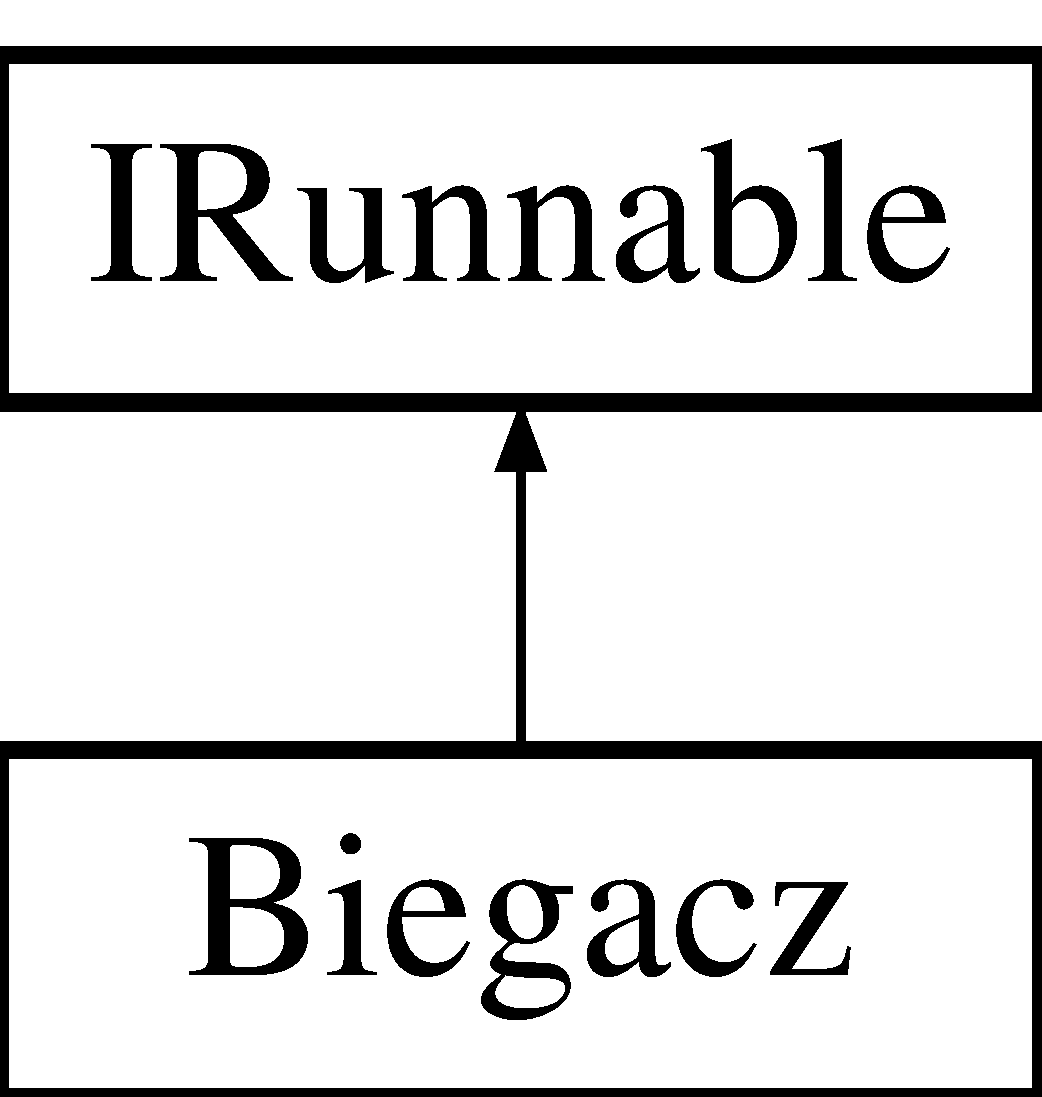
\includegraphics[height=2.000000cm]{class_biegacz}
\end{center}
\end{figure}
\subsection*{Public Member Functions}
\begin{DoxyCompactItemize}
\item 
\hyperlink{class_biegacz_a9d96f7a62f68dc82082242f1171d0c3e}{Biegacz} ()
\item 
virtual \hyperlink{class_biegacz_a76507051a4060a27bdf2867f391fd85b}{$\sim$\-Biegacz} ()
\item 
bool \hyperlink{class_biegacz_a1967974c503d96a81b24f301ca57ee66}{prepare} (int size)
\begin{DoxyCompactList}\small\item\em przygotowanie biegacza, czyli oczyszczenie z tablicy wynikow po wczesniejszym biegu i przygotowanie nowego dystansu. \end{DoxyCompactList}\item 
bool \hyperlink{class_biegacz_a235f4fa4a295a2958b8d8f05f276515b}{run} ()
\end{DoxyCompactItemize}


\subsection{Detailed Description}


Definition at line 7 of file Biegacz.\-h.



\subsection{Constructor \& Destructor Documentation}
\hypertarget{class_biegacz_a9d96f7a62f68dc82082242f1171d0c3e}{\index{Biegacz@{Biegacz}!Biegacz@{Biegacz}}
\index{Biegacz@{Biegacz}!Biegacz@{Biegacz}}
\subsubsection[{Biegacz}]{\setlength{\rightskip}{0pt plus 5cm}Biegacz\-::\-Biegacz (
\begin{DoxyParamCaption}
{}
\end{DoxyParamCaption}
)}}\label{class_biegacz_a9d96f7a62f68dc82082242f1171d0c3e}
stworzenie tablicy do powiekszenia 

Definition at line 3 of file Biegacz.\-cpp.

\hypertarget{class_biegacz_a76507051a4060a27bdf2867f391fd85b}{\index{Biegacz@{Biegacz}!$\sim$\-Biegacz@{$\sim$\-Biegacz}}
\index{$\sim$\-Biegacz@{$\sim$\-Biegacz}!Biegacz@{Biegacz}}
\subsubsection[{$\sim$\-Biegacz}]{\setlength{\rightskip}{0pt plus 5cm}Biegacz\-::$\sim$\-Biegacz (
\begin{DoxyParamCaption}
{}
\end{DoxyParamCaption}
)\hspace{0.3cm}{\ttfamily [virtual]}}}\label{class_biegacz_a76507051a4060a27bdf2867f391fd85b}


Definition at line 10 of file Biegacz.\-cpp.



\subsection{Member Function Documentation}
\hypertarget{class_biegacz_a1967974c503d96a81b24f301ca57ee66}{\index{Biegacz@{Biegacz}!prepare@{prepare}}
\index{prepare@{prepare}!Biegacz@{Biegacz}}
\subsubsection[{prepare}]{\setlength{\rightskip}{0pt plus 5cm}bool Biegacz\-::prepare (
\begin{DoxyParamCaption}
\item[{int}]{size}
\end{DoxyParamCaption}
)\hspace{0.3cm}{\ttfamily [virtual]}}}\label{class_biegacz_a1967974c503d96a81b24f301ca57ee66}
Sprzatam po poprzednim \char`\"{}biegu\char`\"{}, ustawiam wartosci poczatkowe

oczekiwana wart\-: 10,10$^\wedge$3,10$^\wedge$5... 

Implements \hyperlink{class_i_runnable_ab4916d02d90d684028529fabbf76224b}{I\-Runnable}.



Definition at line 50 of file Biegacz.\-cpp.

\hypertarget{class_biegacz_a235f4fa4a295a2958b8d8f05f276515b}{\index{Biegacz@{Biegacz}!run@{run}}
\index{run@{run}!Biegacz@{Biegacz}}
\subsubsection[{run}]{\setlength{\rightskip}{0pt plus 5cm}bool Biegacz\-::run (
\begin{DoxyParamCaption}
{}
\end{DoxyParamCaption}
)\hspace{0.3cm}{\ttfamily [virtual]}}}\label{class_biegacz_a235f4fa4a295a2958b8d8f05f276515b}
uzupelnianie tablicy zerami. 

Implements \hyperlink{class_i_runnable_ae022a87afe9509ad08d21cda36a4e357}{I\-Runnable}.



Definition at line 61 of file Biegacz.\-cpp.



The documentation for this class was generated from the following files\-:\begin{DoxyCompactItemize}
\item 
/home/patr95/\-Pulpit/\-P\-A\-M\-S\-I/1403/prog/prj/inc/\hyperlink{_biegacz_8h}{Biegacz.\-h}\item 
/home/patr95/\-Pulpit/\-P\-A\-M\-S\-I/1403/prog/prj/src/\hyperlink{_biegacz_8cpp}{Biegacz.\-cpp}\end{DoxyCompactItemize}

\hypertarget{class_biegacz_lista}{\section{Biegacz\-Lista Class Reference}
\label{class_biegacz_lista}\index{Biegacz\-Lista@{Biegacz\-Lista}}
}


Przygotowuje liste i definiuje przebieg jej uzupelniania.  




{\ttfamily \#include $<$Biegacz\-Lista.\-h$>$}

Inheritance diagram for Biegacz\-Lista\-:\begin{figure}[H]
\begin{center}
\leavevmode
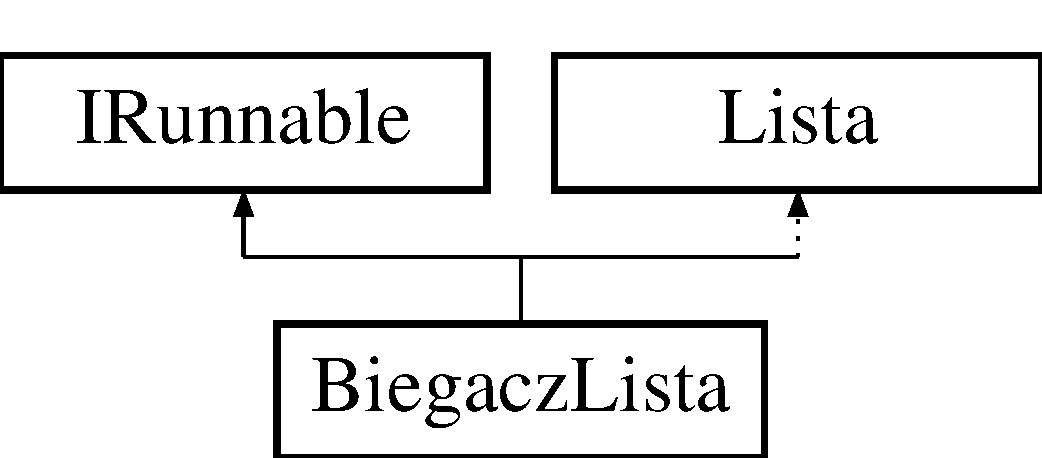
\includegraphics[height=2.000000cm]{class_biegacz_lista}
\end{center}
\end{figure}
\subsection*{Public Member Functions}
\begin{DoxyCompactItemize}
\item 
bool \hyperlink{class_biegacz_lista_a52e49f11f47e35cb0cda910c4ab8f706}{prepare} (int rozmiar\-\_\-docelowy)
\item 
bool \hyperlink{class_biegacz_lista_a6bc929cc4a575a7ef3415e9e8d728f3d}{run} ()
\end{DoxyCompactItemize}


\subsection{Detailed Description}


Definition at line 10 of file Biegacz\-Lista.\-h.



\subsection{Member Function Documentation}
\hypertarget{class_biegacz_lista_a52e49f11f47e35cb0cda910c4ab8f706}{\index{Biegacz\-Lista@{Biegacz\-Lista}!prepare@{prepare}}
\index{prepare@{prepare}!BiegaczLista@{Biegacz\-Lista}}
\subsubsection[{prepare}]{\setlength{\rightskip}{0pt plus 5cm}bool Biegacz\-Lista\-::prepare (
\begin{DoxyParamCaption}
\item[{int}]{rozmiar\-\_\-docelowy}
\end{DoxyParamCaption}
)\hspace{0.3cm}{\ttfamily [virtual]}}}\label{class_biegacz_lista_a52e49f11f47e35cb0cda910c4ab8f706}
Klasa pomocnicza majaca na celu zdefiniowanie metod z tablicowego Biegacza, dla listy. Usuwa wczesniej modyfikowana liste. Funkcja prepare zwieksza rozmiar listy do rozmiaru docelowego, wypelnia ja losowymi slowami, oraz jednym slowem ktorego bedziemy szukac. sprztanie po poprzedniej liscie.

wypelnienie listy losowymi slowami/elementami(stale)

wrzucanie wyrazu na losowe miejsce w liscie 

Implements \hyperlink{class_i_runnable_ab4916d02d90d684028529fabbf76224b}{I\-Runnable}.



Definition at line 3 of file Biegacz\-Lista.\-cpp.

\hypertarget{class_biegacz_lista_a6bc929cc4a575a7ef3415e9e8d728f3d}{\index{Biegacz\-Lista@{Biegacz\-Lista}!run@{run}}
\index{run@{run}!BiegaczLista@{Biegacz\-Lista}}
\subsubsection[{run}]{\setlength{\rightskip}{0pt plus 5cm}bool Biegacz\-Lista\-::run (
\begin{DoxyParamCaption}
{}
\end{DoxyParamCaption}
)\hspace{0.3cm}{\ttfamily [virtual]}}}\label{class_biegacz_lista_a6bc929cc4a575a7ef3415e9e8d728f3d}
Funkcja run wyszukuje slowo i zwraca prawde lub falsz w zaleznosci ,czy znalazlo czy nie. przeszukuje liste by znalezc slowo podane nizej. 

Implements \hyperlink{class_i_runnable_ae022a87afe9509ad08d21cda36a4e357}{I\-Runnable}.



Definition at line 21 of file Biegacz\-Lista.\-cpp.



The documentation for this class was generated from the following files\-:\begin{DoxyCompactItemize}
\item 
/home/patr95/\-Pulpit/\-P\-A\-M\-S\-I/1403/prog/prj/inc/\hyperlink{_biegacz_lista_8h}{Biegacz\-Lista.\-h}\item 
/home/patr95/\-Pulpit/\-P\-A\-M\-S\-I/1403/prog/prj/src/\hyperlink{_biegacz_lista_8cpp}{Biegacz\-Lista.\-cpp}\end{DoxyCompactItemize}

\hypertarget{class_i_lista}{\section{I\-Lista Class Reference}
\label{class_i_lista}\index{I\-Lista@{I\-Lista}}
}


{\ttfamily \#include $<$I\-Lista.\-h$>$}

Inheritance diagram for I\-Lista\-:\begin{figure}[H]
\begin{center}
\leavevmode
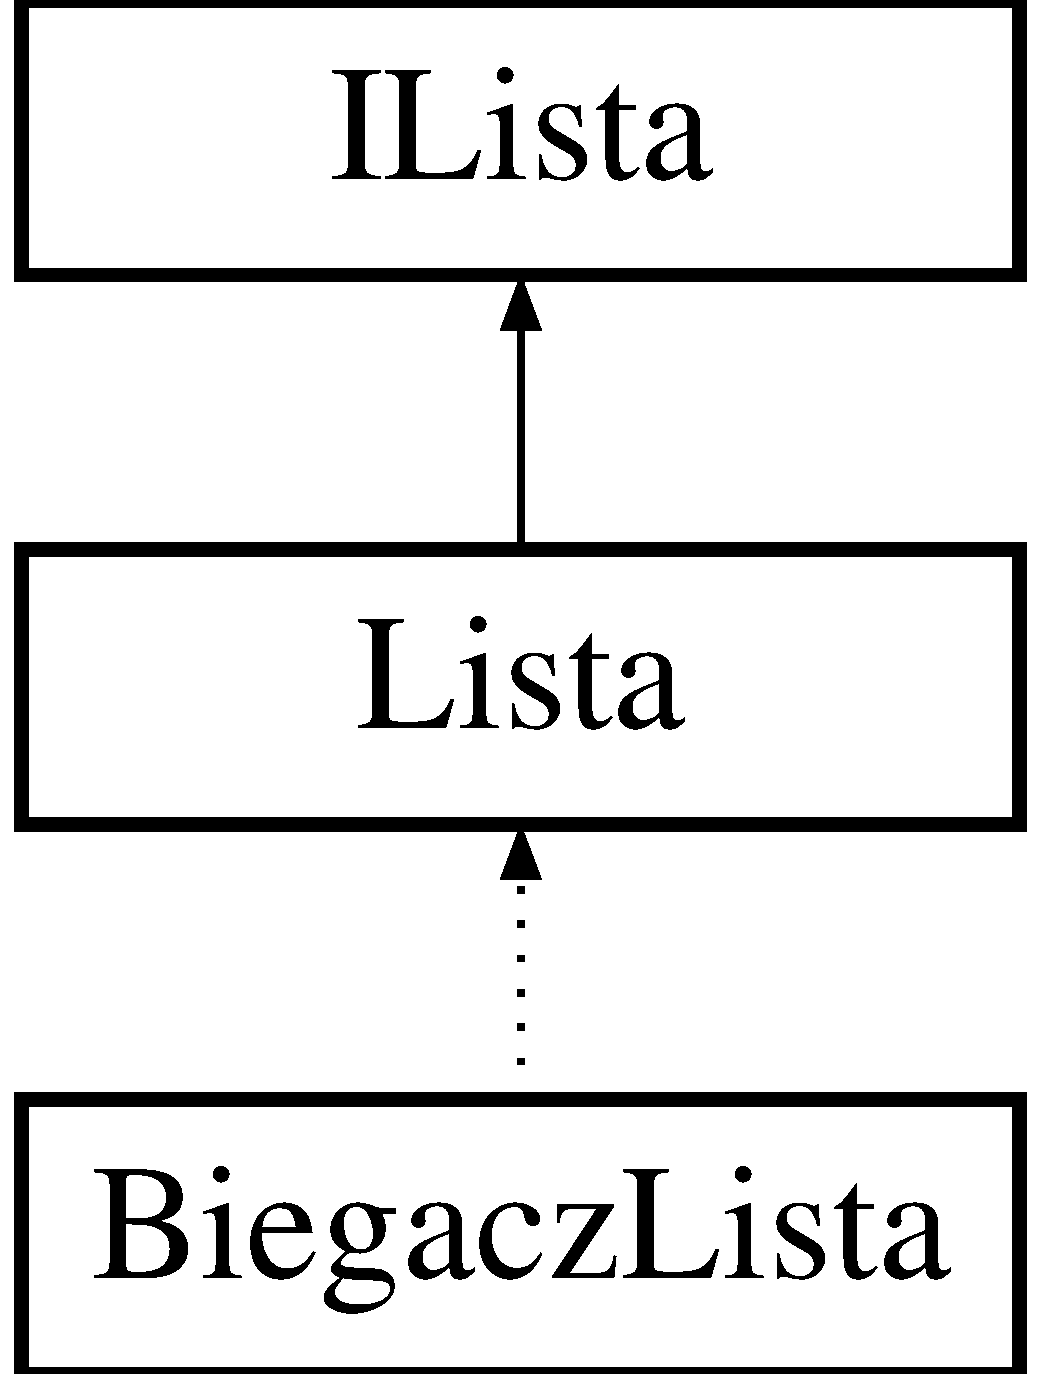
\includegraphics[height=3.000000cm]{class_i_lista}
\end{center}
\end{figure}
\subsection*{Public Member Functions}
\begin{DoxyCompactItemize}
\item 
virtual void \hyperlink{class_i_lista_a0d22daaac5830b397eebfc42547ccb71}{Add} (std\-::string item, int index)=0
\item 
virtual void \hyperlink{class_i_lista_ae2176d09c56106bcff4371785c11ee6f}{Remove} (int index)=0
\item 
virtual bool \hyperlink{class_i_lista_ad2d915eac77a5946d73db20c8695cbab}{Is\-Empty} ()=0
\item 
virtual std\-::string \hyperlink{class_i_lista_a2d9a68dc574d9f059e894c0aae44ab87}{Get} (int index)=0
\item 
virtual int \hyperlink{class_i_lista_a7063d86e7bc765b929ff9d0e0eefa2d1}{Size} ()=0
\end{DoxyCompactItemize}


\subsection{Detailed Description}


Definition at line 5 of file I\-Lista.\-h.



\subsection{Member Function Documentation}
\hypertarget{class_i_lista_a0d22daaac5830b397eebfc42547ccb71}{\index{I\-Lista@{I\-Lista}!Add@{Add}}
\index{Add@{Add}!ILista@{I\-Lista}}
\subsubsection[{Add}]{\setlength{\rightskip}{0pt plus 5cm}virtual void I\-Lista\-::\-Add (
\begin{DoxyParamCaption}
\item[{std\-::string}]{item, }
\item[{int}]{index}
\end{DoxyParamCaption}
)\hspace{0.3cm}{\ttfamily [pure virtual]}}}\label{class_i_lista_a0d22daaac5830b397eebfc42547ccb71}


Implemented in \hyperlink{class_lista_a9e4d70d858b6e3a646f180457b09aa04}{Lista}.

\hypertarget{class_i_lista_a2d9a68dc574d9f059e894c0aae44ab87}{\index{I\-Lista@{I\-Lista}!Get@{Get}}
\index{Get@{Get}!ILista@{I\-Lista}}
\subsubsection[{Get}]{\setlength{\rightskip}{0pt plus 5cm}virtual std\-::string I\-Lista\-::\-Get (
\begin{DoxyParamCaption}
\item[{int}]{index}
\end{DoxyParamCaption}
)\hspace{0.3cm}{\ttfamily [pure virtual]}}}\label{class_i_lista_a2d9a68dc574d9f059e894c0aae44ab87}


Implemented in \hyperlink{class_lista_a46ae62bf7552a2350d8680ba95133a4f}{Lista}.

\hypertarget{class_i_lista_ad2d915eac77a5946d73db20c8695cbab}{\index{I\-Lista@{I\-Lista}!Is\-Empty@{Is\-Empty}}
\index{Is\-Empty@{Is\-Empty}!ILista@{I\-Lista}}
\subsubsection[{Is\-Empty}]{\setlength{\rightskip}{0pt plus 5cm}virtual bool I\-Lista\-::\-Is\-Empty (
\begin{DoxyParamCaption}
{}
\end{DoxyParamCaption}
)\hspace{0.3cm}{\ttfamily [pure virtual]}}}\label{class_i_lista_ad2d915eac77a5946d73db20c8695cbab}


Implemented in \hyperlink{class_lista_acceb965602ca6cef206046d40c629395}{Lista}.

\hypertarget{class_i_lista_ae2176d09c56106bcff4371785c11ee6f}{\index{I\-Lista@{I\-Lista}!Remove@{Remove}}
\index{Remove@{Remove}!ILista@{I\-Lista}}
\subsubsection[{Remove}]{\setlength{\rightskip}{0pt plus 5cm}virtual void I\-Lista\-::\-Remove (
\begin{DoxyParamCaption}
\item[{int}]{index}
\end{DoxyParamCaption}
)\hspace{0.3cm}{\ttfamily [pure virtual]}}}\label{class_i_lista_ae2176d09c56106bcff4371785c11ee6f}


Implemented in \hyperlink{class_lista_a6c0bd5efbb3cba185a35bd2aa75beb4d}{Lista}.

\hypertarget{class_i_lista_a7063d86e7bc765b929ff9d0e0eefa2d1}{\index{I\-Lista@{I\-Lista}!Size@{Size}}
\index{Size@{Size}!ILista@{I\-Lista}}
\subsubsection[{Size}]{\setlength{\rightskip}{0pt plus 5cm}virtual int I\-Lista\-::\-Size (
\begin{DoxyParamCaption}
{}
\end{DoxyParamCaption}
)\hspace{0.3cm}{\ttfamily [pure virtual]}}}\label{class_i_lista_a7063d86e7bc765b929ff9d0e0eefa2d1}


Implemented in \hyperlink{class_lista_abdcf8dfca8c018469b53c30433f7062c}{Lista}.



The documentation for this class was generated from the following file\-:\begin{DoxyCompactItemize}
\item 
/home/patr95/\-Pulpit/\-P\-A\-M\-S\-I/1403/prog/prj/inc/\hyperlink{_i_lista_8h}{I\-Lista.\-h}\end{DoxyCompactItemize}

\hypertarget{class_i_runnable}{\section{I\-Runnable Class Reference}
\label{class_i_runnable}\index{I\-Runnable@{I\-Runnable}}
}


{\ttfamily \#include $<$I\-Runnable.\-h$>$}

Inheritance diagram for I\-Runnable\-:\begin{figure}[H]
\begin{center}
\leavevmode
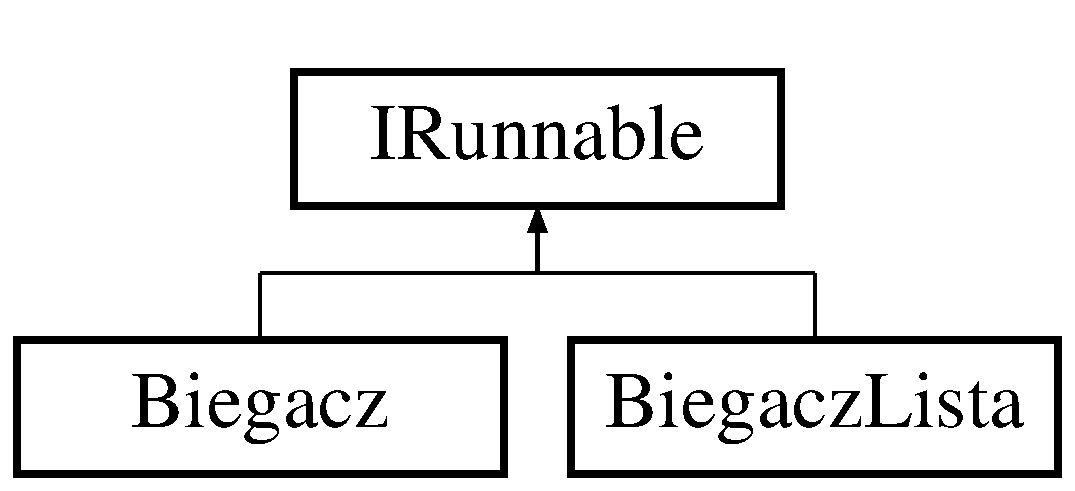
\includegraphics[height=2.000000cm]{class_i_runnable}
\end{center}
\end{figure}
\subsection*{Public Member Functions}
\begin{DoxyCompactItemize}
\item 
virtual bool \hyperlink{class_i_runnable_ab4916d02d90d684028529fabbf76224b}{prepare} (int size)=0
\item 
virtual bool \hyperlink{class_i_runnable_ae022a87afe9509ad08d21cda36a4e357}{run} ()=0
\end{DoxyCompactItemize}


\subsection{Detailed Description}


Definition at line 3 of file I\-Runnable.\-h.



\subsection{Member Function Documentation}
\hypertarget{class_i_runnable_ab4916d02d90d684028529fabbf76224b}{\index{I\-Runnable@{I\-Runnable}!prepare@{prepare}}
\index{prepare@{prepare}!IRunnable@{I\-Runnable}}
\subsubsection[{prepare}]{\setlength{\rightskip}{0pt plus 5cm}virtual bool I\-Runnable\-::prepare (
\begin{DoxyParamCaption}
\item[{int}]{size}
\end{DoxyParamCaption}
)\hspace{0.3cm}{\ttfamily [pure virtual]}}}\label{class_i_runnable_ab4916d02d90d684028529fabbf76224b}


Implemented in \hyperlink{class_biegacz_a1967974c503d96a81b24f301ca57ee66}{Biegacz}, and \hyperlink{class_biegacz_lista_a52e49f11f47e35cb0cda910c4ab8f706}{Biegacz\-Lista}.

\hypertarget{class_i_runnable_ae022a87afe9509ad08d21cda36a4e357}{\index{I\-Runnable@{I\-Runnable}!run@{run}}
\index{run@{run}!IRunnable@{I\-Runnable}}
\subsubsection[{run}]{\setlength{\rightskip}{0pt plus 5cm}virtual bool I\-Runnable\-::run (
\begin{DoxyParamCaption}
{}
\end{DoxyParamCaption}
)\hspace{0.3cm}{\ttfamily [pure virtual]}}}\label{class_i_runnable_ae022a87afe9509ad08d21cda36a4e357}


Implemented in \hyperlink{class_biegacz_a235f4fa4a295a2958b8d8f05f276515b}{Biegacz}, and \hyperlink{class_biegacz_lista_a6bc929cc4a575a7ef3415e9e8d728f3d}{Biegacz\-Lista}.



The documentation for this class was generated from the following file\-:\begin{DoxyCompactItemize}
\item 
/home/patr95/\-Pulpit/\-P\-A\-M\-S\-I/1403/prog/prj/inc/\hyperlink{_i_runnable_8h}{I\-Runnable.\-h}\end{DoxyCompactItemize}

\hypertarget{class_i_stoper}{\section{I\-Stoper Class Reference}
\label{class_i_stoper}\index{I\-Stoper@{I\-Stoper}}
}


{\ttfamily \#include $<$I\-Stoper.\-h$>$}

Inheritance diagram for I\-Stoper\-:\begin{figure}[H]
\begin{center}
\leavevmode
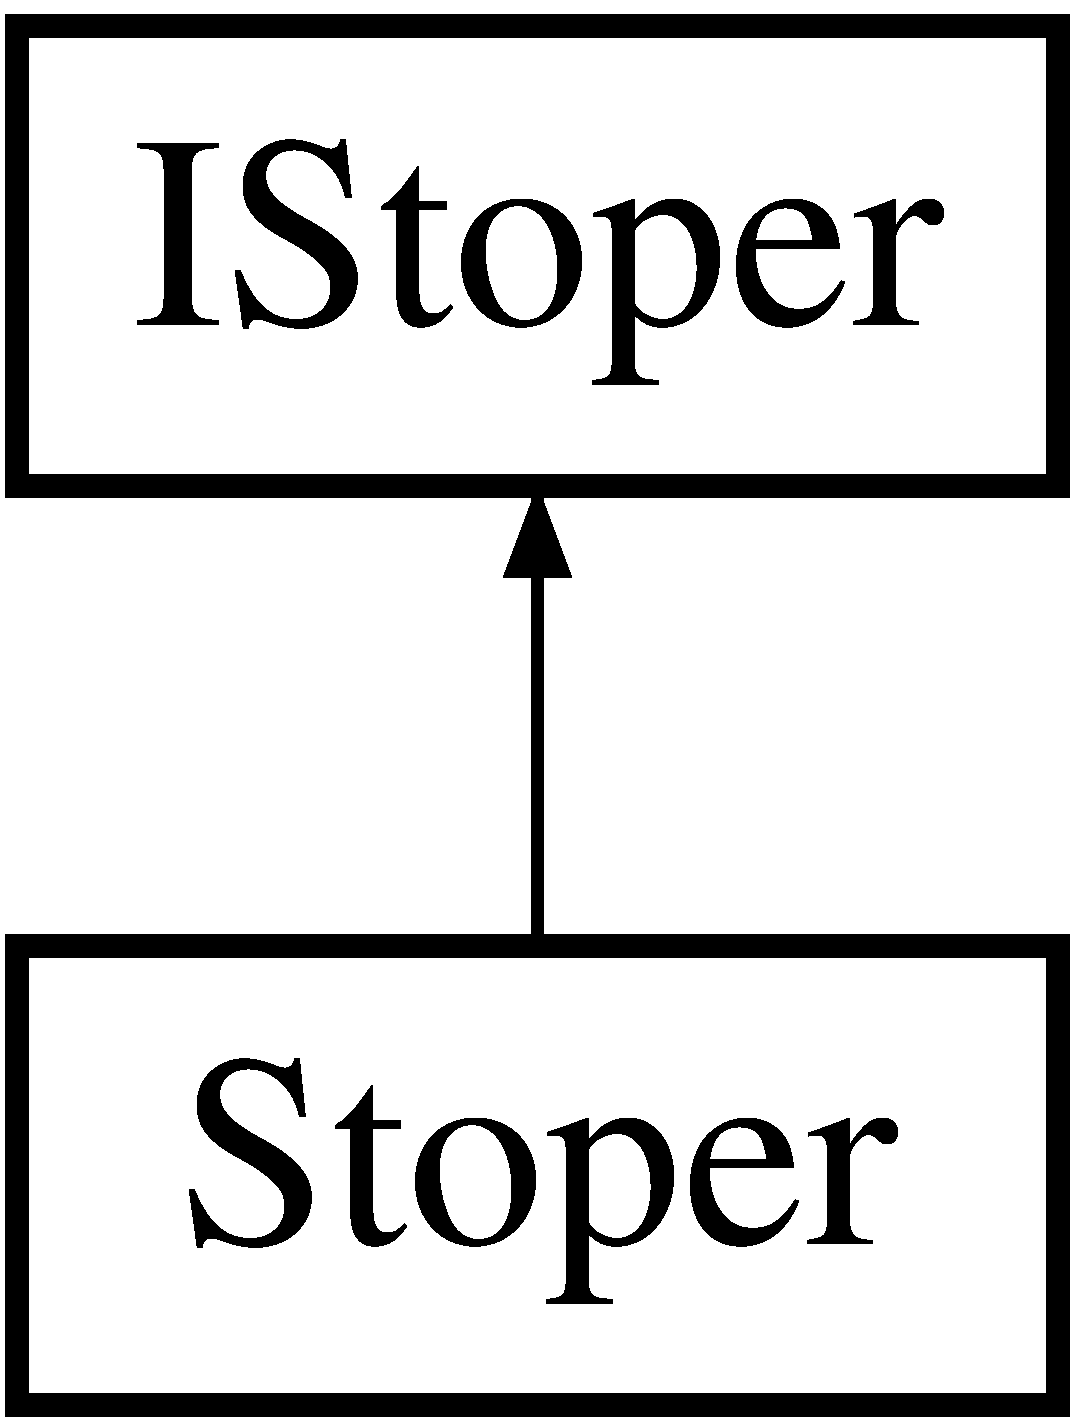
\includegraphics[height=2.000000cm]{class_i_stoper}
\end{center}
\end{figure}
\subsection*{Public Member Functions}
\begin{DoxyCompactItemize}
\item 
virtual void \hyperlink{class_i_stoper_af250c507e0525d290751e0d8e8b3f4b4}{Start} ()=0
\item 
virtual void \hyperlink{class_i_stoper_a185e9c07e0376eb2075f4549ef166243}{Stop} ()=0
\item 
virtual double \hyperlink{class_i_stoper_abf0cb1128747e1a482ed487af6e6d114}{get\-Elapsed\-Time} ()=0
\item 
virtual void \hyperlink{class_i_stoper_a7b0d30f85063cc2171197d93d8a0de5d}{dump\-To\-File} (std\-::string const \&)=0
\end{DoxyCompactItemize}


\subsection{Detailed Description}


Definition at line 5 of file I\-Stoper.\-h.



\subsection{Member Function Documentation}
\hypertarget{class_i_stoper_a7b0d30f85063cc2171197d93d8a0de5d}{\index{I\-Stoper@{I\-Stoper}!dump\-To\-File@{dump\-To\-File}}
\index{dump\-To\-File@{dump\-To\-File}!IStoper@{I\-Stoper}}
\subsubsection[{dump\-To\-File}]{\setlength{\rightskip}{0pt plus 5cm}virtual void I\-Stoper\-::dump\-To\-File (
\begin{DoxyParamCaption}
\item[{std\-::string const \&}]{}
\end{DoxyParamCaption}
)\hspace{0.3cm}{\ttfamily [pure virtual]}}}\label{class_i_stoper_a7b0d30f85063cc2171197d93d8a0de5d}


Implemented in \hyperlink{class_stoper_a4a5dd13c26112cb43b11203fe9f7d4a7}{Stoper}.

\hypertarget{class_i_stoper_abf0cb1128747e1a482ed487af6e6d114}{\index{I\-Stoper@{I\-Stoper}!get\-Elapsed\-Time@{get\-Elapsed\-Time}}
\index{get\-Elapsed\-Time@{get\-Elapsed\-Time}!IStoper@{I\-Stoper}}
\subsubsection[{get\-Elapsed\-Time}]{\setlength{\rightskip}{0pt plus 5cm}virtual double I\-Stoper\-::get\-Elapsed\-Time (
\begin{DoxyParamCaption}
{}
\end{DoxyParamCaption}
)\hspace{0.3cm}{\ttfamily [pure virtual]}}}\label{class_i_stoper_abf0cb1128747e1a482ed487af6e6d114}


Implemented in \hyperlink{class_stoper_a8f50bbba9cb719ca9d573a5cb4a19e36}{Stoper}.

\hypertarget{class_i_stoper_af250c507e0525d290751e0d8e8b3f4b4}{\index{I\-Stoper@{I\-Stoper}!Start@{Start}}
\index{Start@{Start}!IStoper@{I\-Stoper}}
\subsubsection[{Start}]{\setlength{\rightskip}{0pt plus 5cm}virtual void I\-Stoper\-::\-Start (
\begin{DoxyParamCaption}
{}
\end{DoxyParamCaption}
)\hspace{0.3cm}{\ttfamily [pure virtual]}}}\label{class_i_stoper_af250c507e0525d290751e0d8e8b3f4b4}


Implemented in \hyperlink{class_stoper_a5cfc1f0da41e5ca2728e2d80b8da72b9}{Stoper}.

\hypertarget{class_i_stoper_a185e9c07e0376eb2075f4549ef166243}{\index{I\-Stoper@{I\-Stoper}!Stop@{Stop}}
\index{Stop@{Stop}!IStoper@{I\-Stoper}}
\subsubsection[{Stop}]{\setlength{\rightskip}{0pt plus 5cm}virtual void I\-Stoper\-::\-Stop (
\begin{DoxyParamCaption}
{}
\end{DoxyParamCaption}
)\hspace{0.3cm}{\ttfamily [pure virtual]}}}\label{class_i_stoper_a185e9c07e0376eb2075f4549ef166243}


Implemented in \hyperlink{class_stoper_a0890e704c10c35d858490eb68b04df7e}{Stoper}.



The documentation for this class was generated from the following file\-:\begin{DoxyCompactItemize}
\item 
/home/patr95/\-Pulpit/\-P\-A\-M\-S\-I/1403/prog/prj/inc/\hyperlink{_i_stoper_8h}{I\-Stoper.\-h}\end{DoxyCompactItemize}

\hypertarget{class_lista}{\section{Lista Class Reference}
\label{class_lista}\index{Lista@{Lista}}
}


Deklaruje funkcje listy.  




{\ttfamily \#include $<$Lista.\-h$>$}

Inheritance diagram for Lista\-:\begin{figure}[H]
\begin{center}
\leavevmode
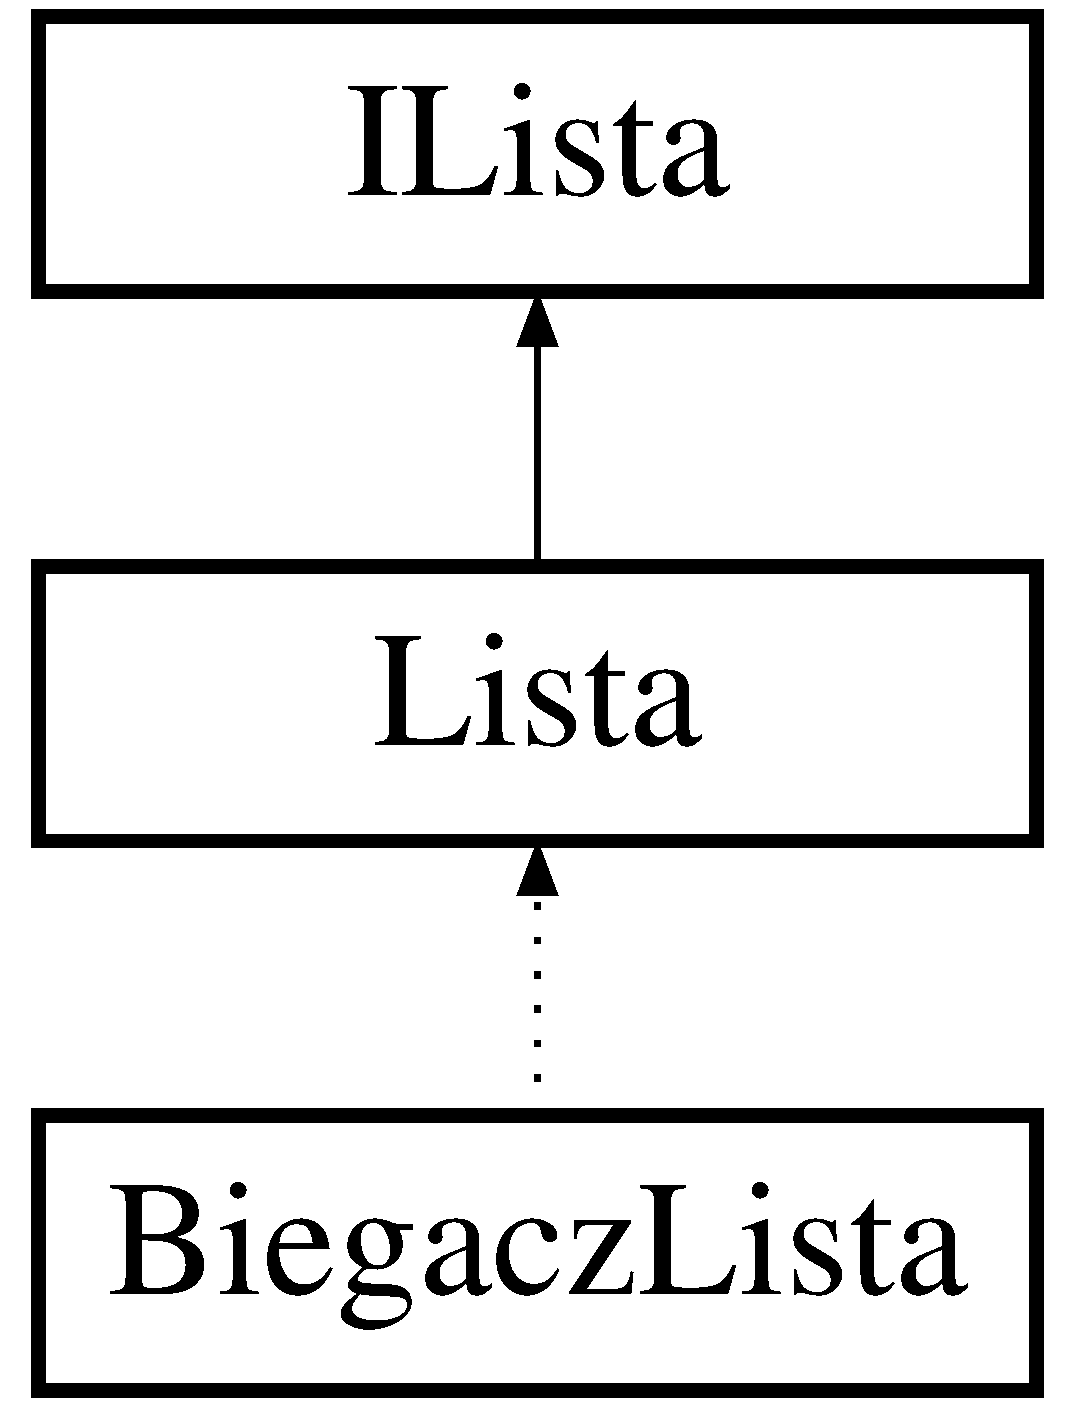
\includegraphics[height=3.000000cm]{class_lista}
\end{center}
\end{figure}
\subsection*{Public Member Functions}
\begin{DoxyCompactItemize}
\item 
void \hyperlink{class_lista_a9e4d70d858b6e3a646f180457b09aa04}{Add} (std\-::string item, int index)
\item 
void \hyperlink{class_lista_a6c0bd5efbb3cba185a35bd2aa75beb4d}{Remove} (int index)
\item 
bool \hyperlink{class_lista_acceb965602ca6cef206046d40c629395}{Is\-Empty} ()
\item 
std\-::string \hyperlink{class_lista_a46ae62bf7552a2350d8680ba95133a4f}{Get} (int index)
\item 
int \hyperlink{class_lista_abdcf8dfca8c018469b53c30433f7062c}{Size} ()
\item 
\hyperlink{class_lista_a1f668b36909182ef1360b48503529a31}{Lista} ()
\end{DoxyCompactItemize}


\subsection{Detailed Description}


Definition at line 17 of file Lista.\-h.



\subsection{Constructor \& Destructor Documentation}
\hypertarget{class_lista_a1f668b36909182ef1360b48503529a31}{\index{Lista@{Lista}!Lista@{Lista}}
\index{Lista@{Lista}!Lista@{Lista}}
\subsubsection[{Lista}]{\setlength{\rightskip}{0pt plus 5cm}Lista\-::\-Lista (
\begin{DoxyParamCaption}
{}
\end{DoxyParamCaption}
)\hspace{0.3cm}{\ttfamily [inline]}}}\label{class_lista_a1f668b36909182ef1360b48503529a31}


Definition at line 62 of file Lista.\-h.



\subsection{Member Function Documentation}
\hypertarget{class_lista_a9e4d70d858b6e3a646f180457b09aa04}{\index{Lista@{Lista}!Add@{Add}}
\index{Add@{Add}!Lista@{Lista}}
\subsubsection[{Add}]{\setlength{\rightskip}{0pt plus 5cm}void Lista\-::\-Add (
\begin{DoxyParamCaption}
\item[{std\-::string}]{item, }
\item[{int}]{index}
\end{DoxyParamCaption}
)\hspace{0.3cm}{\ttfamily [virtual]}}}\label{class_lista_a9e4d70d858b6e3a646f180457b09aa04}
Funkcja Add dodaje kolejny element listy. Jesli rozmiar listy jest za maly w stosunku do podawanego indexu to wyswietla komunikat. Funkcja dziala w taki sposob, ze tworzy nowy \char`\"{}\-Node\char`\"{} do tablicy, wskaznik z wczesniejszego elementu wskazuje na nowy \hyperlink{struct_node}{Node} nastepnie z \hyperlink{struct_node}{Node} wskazujemy na kolejny element tablicy, aby byla ciaglosc w liscie. W tej funkcji rozpatrujemy 3 przypadki zwieksznaia listy, dostawianie elementu na pocz,koniec lub gdzies pomiedzy w liscie. Jesli dostawiamy na poczatek tworzymy nowy element i wskazujemy na niego wskaznikiem poczatkowym i koncowym. Jesli tworzymy ostatni element, to dodajemy nowego Noda, i wskazujemy na niego wskaznikiem\-K\-O\-Ncowym. Osttanim przypadkiem jest elementu gdzies pomiedzy P\-O\-C\-Z i K\-O\-N listy. Tutaj musimy pamietac ze lista liczy swojem miejsca od 0, wiec w petli for mamy index-\/1. Tworzymy tymczasowy wskaznik i ustawiamy go na pierwszy element. nastepnie w petli przesówamy o tyle elementów ile zadamy-\/1. Przesuwamy ten wskaznik na kolejny element, tworzymy pomocniczy wskaznik ktory ma wskazywac na nowo utworzony element. W nowo utworzonym elemencie dodajemy wskaznik ktory wskazuje na nastepny element ktory byl stworzony przed naszym nowym Nodem.\-Wszystko po to by zachowac ciaglosc listy i wskazywanie na kolejne elementy. dostawiam element na poczatku i wskazuje na wczesniejszy element

aktualizowanie poczatkowoego wskaznika na nowo dodany element

aktualizowanie koncowego+ wskaznika na nowo dodany element

wskaznik koncowy wskazuje na podpiete nowe pole w liscie

temp to tymczasowy wskaznik dodawanej listy

przestawiamy sie na kolejny element

pomocniczy wskaznik

wskazuje na nowo stworzony element

w nowo dodanym elemencie ustawiamy wskaznik na wczesniejszy(ktory jest nastepnym) elementem. 

Implements \hyperlink{class_i_lista_a0d22daaac5830b397eebfc42547ccb71}{I\-Lista}.



Definition at line 12 of file Lista.\-cpp.

\hypertarget{class_lista_a46ae62bf7552a2350d8680ba95133a4f}{\index{Lista@{Lista}!Get@{Get}}
\index{Get@{Get}!Lista@{Lista}}
\subsubsection[{Get}]{\setlength{\rightskip}{0pt plus 5cm}std\-::string Lista\-::\-Get (
\begin{DoxyParamCaption}
\item[{int}]{index}
\end{DoxyParamCaption}
)\hspace{0.3cm}{\ttfamily [virtual]}}}\label{class_lista_a46ae62bf7552a2350d8680ba95133a4f}
W tej funkcji tworzymy wskaznik tymczasowy na 1 element listy, przesuwamy o index-\/1 , po znalezieniu interesujacego nas elementu zwracamy jego wartosc. temp to tymczasowy wskaznik dodawanej listy 

Implements \hyperlink{class_i_lista_a2d9a68dc574d9f059e894c0aae44ab87}{I\-Lista}.



Definition at line 70 of file Lista.\-cpp.

\hypertarget{class_lista_acceb965602ca6cef206046d40c629395}{\index{Lista@{Lista}!Is\-Empty@{Is\-Empty}}
\index{Is\-Empty@{Is\-Empty}!Lista@{Lista}}
\subsubsection[{Is\-Empty}]{\setlength{\rightskip}{0pt plus 5cm}bool Lista\-::\-Is\-Empty (
\begin{DoxyParamCaption}
{}
\end{DoxyParamCaption}
)\hspace{0.3cm}{\ttfamily [virtual]}}}\label{class_lista_acceb965602ca6cef206046d40c629395}
Zwraca true jesli lista jest pusta lub false jesli nie jest. 

Implements \hyperlink{class_i_lista_ad2d915eac77a5946d73db20c8695cbab}{I\-Lista}.



Definition at line 8 of file Lista.\-cpp.

\hypertarget{class_lista_a6c0bd5efbb3cba185a35bd2aa75beb4d}{\index{Lista@{Lista}!Remove@{Remove}}
\index{Remove@{Remove}!Lista@{Lista}}
\subsubsection[{Remove}]{\setlength{\rightskip}{0pt plus 5cm}void Lista\-::\-Remove (
\begin{DoxyParamCaption}
\item[{int}]{index}
\end{DoxyParamCaption}
)\hspace{0.3cm}{\ttfamily [virtual]}}}\label{class_lista_a6c0bd5efbb3cba185a35bd2aa75beb4d}
Remove dziala w podobny sposob. Jesli zadamy usuniecie 1 elementu, to zapamietujemy cos na co wskazuje 1 element. Usuwamy to, by nastepnie ustawic wskaznik poczatkowy na cos, na co wskazywal pierwszy element. Jesli usuwamy ostatni element to tworzymy wskaznik tymczasowy na pierwszy element, przesuwamy do ostatniego, gdzie index zmniejszamy -\/2, poniewaz indexujemy liste od zera, oraz interesuje nas wczesniejszy element ktory wskazuje na ostatni. Gdy osiegniey przedostatni element wskazujemy jego wskaznikiem na null pointer oraz usuwamy wczesniejszy osttni element z listy na ktorego nic nie wskazuje. W ostatnim przypadku tworzymy tymczasowy nastepnik , ktory jest wskaznikiem na wskaznik. Przesukujemy liste od poczatku, usuwamy element i nasz wskaznik dalej wskazuje na kolejny element dzieki nastepnikowi. Zachowana jest ciaglosc wskazywania na siebie elementow z listy. zapamietaj drugi element listy

usun pierwszy element

przestaw drugi na pierwszy

temp to tymczasowy wskaznik dodawanej listy

przestawiamy sie na kolejny element

temp to tymczasowy wskaznik dodawanej listy 

Implements \hyperlink{class_i_lista_ae2176d09c56106bcff4371785c11ee6f}{I\-Lista}.



Definition at line 43 of file Lista.\-cpp.

\hypertarget{class_lista_abdcf8dfca8c018469b53c30433f7062c}{\index{Lista@{Lista}!Size@{Size}}
\index{Size@{Size}!Lista@{Lista}}
\subsubsection[{Size}]{\setlength{\rightskip}{0pt plus 5cm}int Lista\-::\-Size (
\begin{DoxyParamCaption}
{}
\end{DoxyParamCaption}
)\hspace{0.3cm}{\ttfamily [virtual]}}}\label{class_lista_abdcf8dfca8c018469b53c30433f7062c}
Size zwraca nam zmienna rozmiar. 

Implements \hyperlink{class_i_lista_a7063d86e7bc765b929ff9d0e0eefa2d1}{I\-Lista}.



Definition at line 3 of file Lista.\-cpp.



The documentation for this class was generated from the following files\-:\begin{DoxyCompactItemize}
\item 
/home/patr95/\-Pulpit/\-P\-A\-M\-S\-I/1403/prog/prj/inc/\hyperlink{_lista_8h}{Lista.\-h}\item 
/home/patr95/\-Pulpit/\-P\-A\-M\-S\-I/1403/prog/prj/src/\hyperlink{_lista_8cpp}{Lista.\-cpp}\end{DoxyCompactItemize}

\hypertarget{struct_node}{\section{Node Struct Reference}
\label{struct_node}\index{Node@{Node}}
}


pojedynczy element  




{\ttfamily \#include $<$Lista.\-h$>$}

\subsection*{Public Attributes}
\begin{DoxyCompactItemize}
\item 
\hyperlink{struct_node}{Node} $\ast$ \hyperlink{struct_node_a738fc042ebfbe87177d8b3dbf9b7ba8e}{wskaznik}
\item 
std\-::string \hyperlink{struct_node_a27b5f552615a84991370e185f4390fba}{wartosc}
\end{DoxyCompactItemize}


\subsection{Detailed Description}


Definition at line 8 of file Lista.\-h.



\subsection{Member Data Documentation}
\hypertarget{struct_node_a27b5f552615a84991370e185f4390fba}{\index{Node@{Node}!wartosc@{wartosc}}
\index{wartosc@{wartosc}!Node@{Node}}
\subsubsection[{wartosc}]{\setlength{\rightskip}{0pt plus 5cm}std\-::string Node\-::wartosc}}\label{struct_node_a27b5f552615a84991370e185f4390fba}


Definition at line 11 of file Lista.\-h.

\hypertarget{struct_node_a738fc042ebfbe87177d8b3dbf9b7ba8e}{\index{Node@{Node}!wskaznik@{wskaznik}}
\index{wskaznik@{wskaznik}!Node@{Node}}
\subsubsection[{wskaznik}]{\setlength{\rightskip}{0pt plus 5cm}{\bf Node}$\ast$ Node\-::wskaznik}}\label{struct_node_a738fc042ebfbe87177d8b3dbf9b7ba8e}


Definition at line 10 of file Lista.\-h.



The documentation for this struct was generated from the following file\-:\begin{DoxyCompactItemize}
\item 
/home/patr95/\-Pulpit/\-P\-A\-M\-S\-I/1403/prog/prj/inc/\hyperlink{_lista_8h}{Lista.\-h}\end{DoxyCompactItemize}

\hypertarget{class_sedzia}{\section{Sedzia Class Reference}
\label{class_sedzia}\index{Sedzia@{Sedzia}}
}


Jest to klasa nadrzedna , ktora struje klasami \hyperlink{class_stoper}{Stoper} i \hyperlink{class_biegacz}{Biegacz} poprzez odwolanie sie do interfejsow.  




{\ttfamily \#include $<$Sedzia.\-h$>$}

\subsection*{Public Member Functions}
\begin{DoxyCompactItemize}
\item 
\hyperlink{class_sedzia_ae4d4ad29d07d9e0b8336fc64a56ee4ee}{Sedzia} (\hyperlink{class_i_runnable}{I\-Runnable} \&biegacz, \hyperlink{class_i_stoper}{I\-Stoper} \&stoper)
\item 
void \hyperlink{class_sedzia_a21336aaef6c5e2476605468aee086079}{release} ()
\end{DoxyCompactItemize}


\subsection{Detailed Description}


Definition at line 16 of file Sedzia.\-h.



\subsection{Constructor \& Destructor Documentation}
\hypertarget{class_sedzia_ae4d4ad29d07d9e0b8336fc64a56ee4ee}{\index{Sedzia@{Sedzia}!Sedzia@{Sedzia}}
\index{Sedzia@{Sedzia}!Sedzia@{Sedzia}}
\subsubsection[{Sedzia}]{\setlength{\rightskip}{0pt plus 5cm}Sedzia\-::\-Sedzia (
\begin{DoxyParamCaption}
\item[{{\bf I\-Runnable} \&}]{biegacz, }
\item[{{\bf I\-Stoper} \&}]{stoper}
\end{DoxyParamCaption}
)\hspace{0.3cm}{\ttfamily [inline]}}}\label{class_sedzia_ae4d4ad29d07d9e0b8336fc64a56ee4ee}


Definition at line 21 of file Sedzia.\-h.



\subsection{Member Function Documentation}
\hypertarget{class_sedzia_a21336aaef6c5e2476605468aee086079}{\index{Sedzia@{Sedzia}!release@{release}}
\index{release@{release}!Sedzia@{Sedzia}}
\subsubsection[{release}]{\setlength{\rightskip}{0pt plus 5cm}void Sedzia\-::release (
\begin{DoxyParamCaption}
{}
\end{DoxyParamCaption}
)}}\label{class_sedzia_a21336aaef6c5e2476605468aee086079}
Przez funkcje release wywolujemy kolejno funkcje biegacz prepare-\/$>$Start-\/$>$run-\/$>$Stop-\/$>$get\-Elapsed\-Time-\/$>$dump\-To\-File ktore sa zdefiniowane w klasach \hyperlink{class_stoper}{Stoper} i \hyperlink{class_biegacz}{Biegacz}. Mamy taka mozliwosc poprzez interfejsy. 

Definition at line 3 of file Sedzia.\-cpp.



The documentation for this class was generated from the following files\-:\begin{DoxyCompactItemize}
\item 
/home/patr95/\-Pulpit/\-P\-A\-M\-S\-I/1403/prog/prj/inc/\hyperlink{_sedzia_8h}{Sedzia.\-h}\item 
/home/patr95/\-Pulpit/\-P\-A\-M\-S\-I/1403/prog/prj/src/\hyperlink{_sedzia_8cpp}{Sedzia.\-cpp}\end{DoxyCompactItemize}

\hypertarget{class_stoper}{\section{Stoper Class Reference}
\label{class_stoper}\index{Stoper@{Stoper}}
}


zastepuje kilkukrotne wklejanie pliku naglowkowego  




{\ttfamily \#include $<$Stoper.\-h$>$}

Inheritance diagram for Stoper\-:\begin{figure}[H]
\begin{center}
\leavevmode
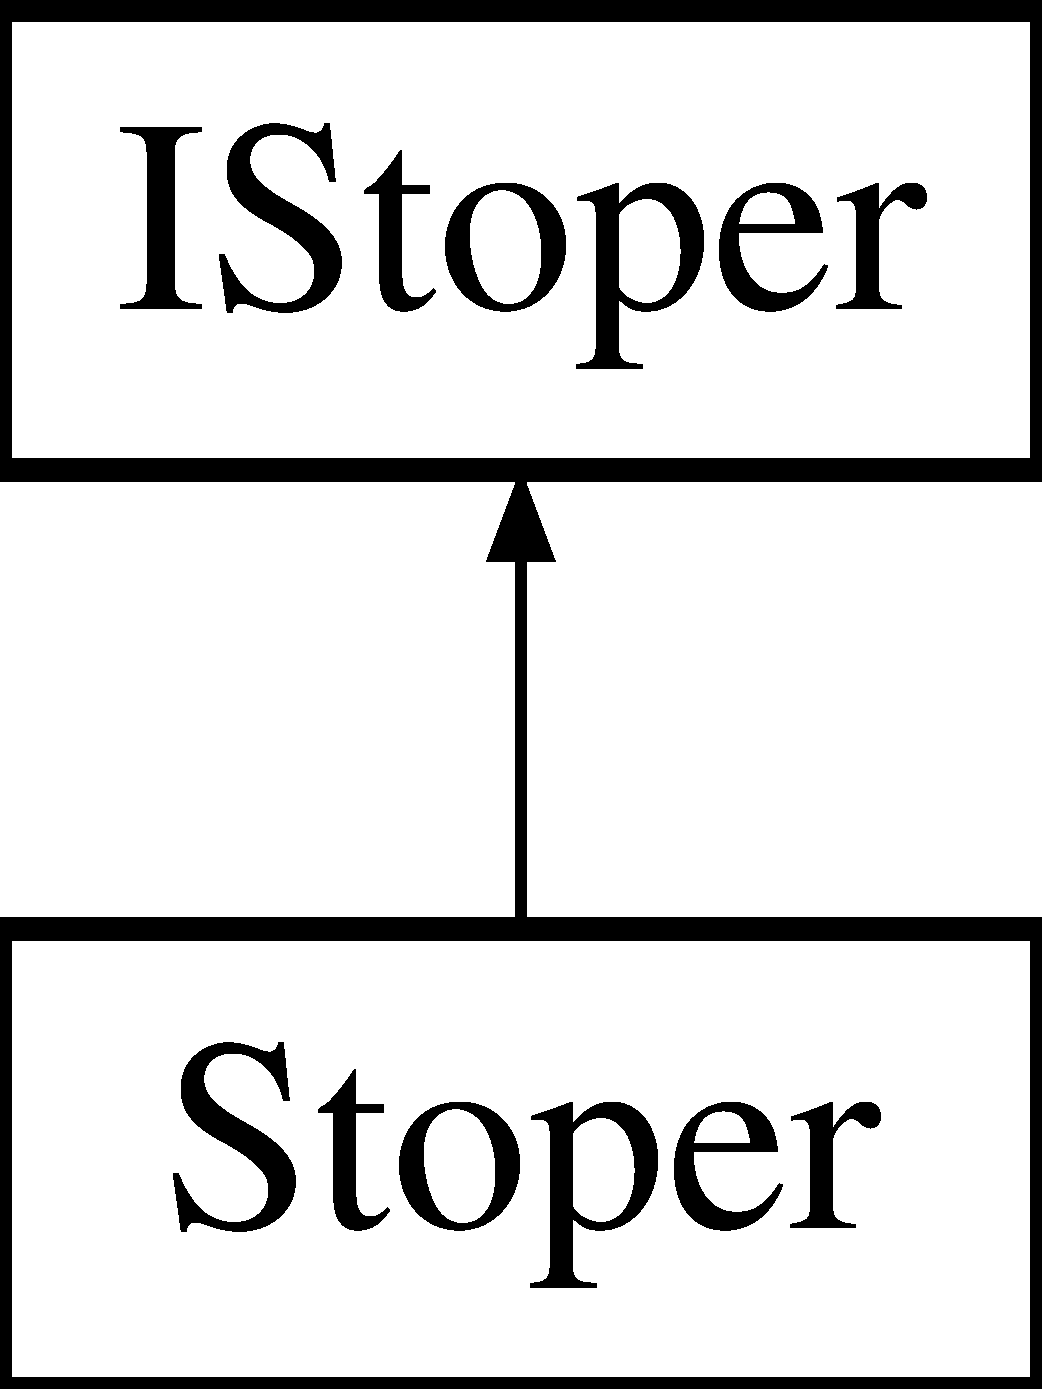
\includegraphics[height=2.000000cm]{class_stoper}
\end{center}
\end{figure}
\subsection*{Public Types}
\begin{DoxyCompactItemize}
\item 
using \hyperlink{class_stoper_ac7b1a0995c65c28a71e3ceabf5c6f965}{clock} = std\-::chrono\-::high\-\_\-resolution\-\_\-clock
\begin{DoxyCompactList}\small\item\em const\& =unikamy kopi \end{DoxyCompactList}\item 
using \hyperlink{class_stoper_a7d5d891cde8e9882bea254614a0fd2dd}{time\-\_\-point} = clock\-::time\-\_\-point
\begin{DoxyCompactList}\small\item\em czas systemowy \end{DoxyCompactList}\item 
using \hyperlink{class_stoper_a249c00c1592a239a8463880dcd657dd3}{time\-\_\-type} = std\-::chrono\-::milliseconds
\end{DoxyCompactItemize}
\subsection*{Public Member Functions}
\begin{DoxyCompactItemize}
\item 
void \hyperlink{class_stoper_a5cfc1f0da41e5ca2728e2d80b8da72b9}{Start} ()
\item 
void \hyperlink{class_stoper_a0890e704c10c35d858490eb68b04df7e}{Stop} ()
\item 
double \hyperlink{class_stoper_a8f50bbba9cb719ca9d573a5cb4a19e36}{get\-Elapsed\-Time} ()
\begin{DoxyCompactList}\small\item\em duration cast=operator porownujacy, pozwala odjac 2 punkty w czasie \end{DoxyCompactList}\item 
void \hyperlink{class_stoper_a4a5dd13c26112cb43b11203fe9f7d4a7}{dump\-To\-File} (std\-::string const \&)
\end{DoxyCompactItemize}


\subsection{Detailed Description}
Mierzy czas,wyswitla czas okrazenia, zwraca wyniki do pliku. 

Definition at line 13 of file Stoper.\-h.



\subsection{Member Typedef Documentation}
\hypertarget{class_stoper_ac7b1a0995c65c28a71e3ceabf5c6f965}{\index{Stoper@{Stoper}!clock@{clock}}
\index{clock@{clock}!Stoper@{Stoper}}
\subsubsection[{clock}]{\setlength{\rightskip}{0pt plus 5cm}using {\bf Stoper\-::clock} =  std\-::chrono\-::high\-\_\-resolution\-\_\-clock}}\label{class_stoper_ac7b1a0995c65c28a71e3ceabf5c6f965}


Definition at line 34 of file Stoper.\-h.

\hypertarget{class_stoper_a7d5d891cde8e9882bea254614a0fd2dd}{\index{Stoper@{Stoper}!time\-\_\-point@{time\-\_\-point}}
\index{time\-\_\-point@{time\-\_\-point}!Stoper@{Stoper}}
\subsubsection[{time\-\_\-point}]{\setlength{\rightskip}{0pt plus 5cm}using {\bf Stoper\-::time\-\_\-point} =  clock\-::time\-\_\-point}}\label{class_stoper_a7d5d891cde8e9882bea254614a0fd2dd}


Definition at line 35 of file Stoper.\-h.

\hypertarget{class_stoper_a249c00c1592a239a8463880dcd657dd3}{\index{Stoper@{Stoper}!time\-\_\-type@{time\-\_\-type}}
\index{time\-\_\-type@{time\-\_\-type}!Stoper@{Stoper}}
\subsubsection[{time\-\_\-type}]{\setlength{\rightskip}{0pt plus 5cm}using {\bf Stoper\-::time\-\_\-type} =  std\-::chrono\-::milliseconds}}\label{class_stoper_a249c00c1592a239a8463880dcd657dd3}


Definition at line 36 of file Stoper.\-h.



\subsection{Member Function Documentation}
\hypertarget{class_stoper_a4a5dd13c26112cb43b11203fe9f7d4a7}{\index{Stoper@{Stoper}!dump\-To\-File@{dump\-To\-File}}
\index{dump\-To\-File@{dump\-To\-File}!Stoper@{Stoper}}
\subsubsection[{dump\-To\-File}]{\setlength{\rightskip}{0pt plus 5cm}void Stoper\-::dump\-To\-File (
\begin{DoxyParamCaption}
\item[{std\-::string const \&}]{nazwa\-Pliku}
\end{DoxyParamCaption}
)\hspace{0.3cm}{\ttfamily [virtual]}}}\label{class_stoper_a4a5dd13c26112cb43b11203fe9f7d4a7}
dump\-To\-File wysyla wyniki do pliku tekstowego. Jesli go nie am to go tworzy. Wyniki wysylane sa w kolejnosci wykonania petli. 

Implements \hyperlink{class_i_stoper_a7b0d30f85063cc2171197d93d8a0de5d}{I\-Stoper}.



Definition at line 19 of file Stoper.\-cpp.

\hypertarget{class_stoper_a8f50bbba9cb719ca9d573a5cb4a19e36}{\index{Stoper@{Stoper}!get\-Elapsed\-Time@{get\-Elapsed\-Time}}
\index{get\-Elapsed\-Time@{get\-Elapsed\-Time}!Stoper@{Stoper}}
\subsubsection[{get\-Elapsed\-Time}]{\setlength{\rightskip}{0pt plus 5cm}double Stoper\-::get\-Elapsed\-Time (
\begin{DoxyParamCaption}
{}
\end{DoxyParamCaption}
)\hspace{0.3cm}{\ttfamily [virtual]}}}\label{class_stoper_a8f50bbba9cb719ca9d573a5cb4a19e36}
get\-Elapsed\-Time wykonuje roznice (Stop-\/\-Start) i zwraca czas w milisekundach 

Implements \hyperlink{class_i_stoper_abf0cb1128747e1a482ed487af6e6d114}{I\-Stoper}.



Definition at line 13 of file Stoper.\-cpp.

\hypertarget{class_stoper_a5cfc1f0da41e5ca2728e2d80b8da72b9}{\index{Stoper@{Stoper}!Start@{Start}}
\index{Start@{Start}!Stoper@{Stoper}}
\subsubsection[{Start}]{\setlength{\rightskip}{0pt plus 5cm}void Stoper\-::\-Start (
\begin{DoxyParamCaption}
{}
\end{DoxyParamCaption}
)\hspace{0.3cm}{\ttfamily [virtual]}}}\label{class_stoper_a5cfc1f0da41e5ca2728e2d80b8da72b9}
Start pobiera czas systemowy przed wykonaniem zadania 

Implements \hyperlink{class_i_stoper_af250c507e0525d290751e0d8e8b3f4b4}{I\-Stoper}.



Definition at line 3 of file Stoper.\-cpp.

\hypertarget{class_stoper_a0890e704c10c35d858490eb68b04df7e}{\index{Stoper@{Stoper}!Stop@{Stop}}
\index{Stop@{Stop}!Stoper@{Stoper}}
\subsubsection[{Stop}]{\setlength{\rightskip}{0pt plus 5cm}void Stoper\-::\-Stop (
\begin{DoxyParamCaption}
{}
\end{DoxyParamCaption}
)\hspace{0.3cm}{\ttfamily [virtual]}}}\label{class_stoper_a0890e704c10c35d858490eb68b04df7e}
Stop pobiera czas systemowy po wykonaniu zadania 

Implements \hyperlink{class_i_stoper_a185e9c07e0376eb2075f4549ef166243}{I\-Stoper}.



Definition at line 8 of file Stoper.\-cpp.



The documentation for this class was generated from the following files\-:\begin{DoxyCompactItemize}
\item 
/home/patr95/\-Pulpit/\-P\-A\-M\-S\-I/1403/prog/prj/inc/\hyperlink{_stoper_8h}{Stoper.\-h}\item 
/home/patr95/\-Pulpit/\-P\-A\-M\-S\-I/1403/prog/prj/src/\hyperlink{_stoper_8cpp}{Stoper.\-cpp}\end{DoxyCompactItemize}

\chapter{File Documentation}
\hypertarget{build_2_c_make_files_22_88_812_82_2_compiler_id_c_2_c_make_c_compiler_id_8c}{\section{/home/patr95/\-Pulpit/\-P\-A\-M\-S\-I/1403/prog/prj/build/\-C\-Make\-Files/2.8.12.2/\-Compiler\-Id\-C/\-C\-Make\-C\-Compiler\-Id.c File Reference}
\label{build_2_c_make_files_22_88_812_82_2_compiler_id_c_2_c_make_c_compiler_id_8c}\index{/home/patr95/\-Pulpit/\-P\-A\-M\-S\-I/1403/prog/prj/build/\-C\-Make\-Files/2.\-8.\-12.\-2/\-Compiler\-Id\-C/\-C\-Make\-C\-Compiler\-Id.\-c@{/home/patr95/\-Pulpit/\-P\-A\-M\-S\-I/1403/prog/prj/build/\-C\-Make\-Files/2.\-8.\-12.\-2/\-Compiler\-Id\-C/\-C\-Make\-C\-Compiler\-Id.\-c}}
}
\subsection*{Macros}
\begin{DoxyCompactItemize}
\item 
\#define \hyperlink{build_2_c_make_files_22_88_812_82_2_compiler_id_c_2_c_make_c_compiler_id_8c_a81dee0709ded976b2e0319239f72d174}{C\-O\-M\-P\-I\-L\-E\-R\-\_\-\-I\-D}~\char`\"{}\char`\"{}
\item 
\#define \hyperlink{build_2_c_make_files_22_88_812_82_2_compiler_id_c_2_c_make_c_compiler_id_8c_adbc5372f40838899018fadbc89bd588b}{P\-L\-A\-T\-F\-O\-R\-M\-\_\-\-I\-D}~\char`\"{}\char`\"{}
\item 
\#define \hyperlink{build_2_c_make_files_22_88_812_82_2_compiler_id_c_2_c_make_c_compiler_id_8c_aba35d0d200deaeb06aee95ca297acb28}{A\-R\-C\-H\-I\-T\-E\-C\-T\-U\-R\-E\-\_\-\-I\-D}~\char`\"{}\char`\"{}
\item 
\#define \hyperlink{build_2_c_make_files_22_88_812_82_2_compiler_id_c_2_c_make_c_compiler_id_8c_ad1280362da42492bbc11aa78cbf776ad}{D\-E\-C}(n)
\item 
\#define \hyperlink{build_2_c_make_files_22_88_812_82_2_compiler_id_c_2_c_make_c_compiler_id_8c_a46d5d95daa1bef867bd0179594310ed5}{H\-E\-X}(n)
\end{DoxyCompactItemize}
\subsection*{Functions}
\begin{DoxyCompactItemize}
\item 
int \hyperlink{build_2_c_make_files_22_88_812_82_2_compiler_id_c_2_c_make_c_compiler_id_8c_a0ddf1224851353fc92bfbff6f499fa97}{main} (int argc, char $\ast$argv\mbox{[}$\,$\mbox{]})
\end{DoxyCompactItemize}
\subsection*{Variables}
\begin{DoxyCompactItemize}
\item 
char const $\ast$ \hyperlink{build_2_c_make_files_22_88_812_82_2_compiler_id_c_2_c_make_c_compiler_id_8c_a4b0efeb7a5d59313986b3a0390f050f6}{info\-\_\-compiler} = \char`\"{}I\-N\-F\-O\char`\"{} \char`\"{}\-:\char`\"{} \char`\"{}compiler\mbox{[}\char`\"{} C\-O\-M\-P\-I\-L\-E\-R\-\_\-\-I\-D \char`\"{}\mbox{]}\char`\"{}
\item 
char const $\ast$ \hyperlink{build_2_c_make_files_22_88_812_82_2_compiler_id_c_2_c_make_c_compiler_id_8c_a2321403dee54ee23f0c2fa849c60f7d4}{info\-\_\-platform} = \char`\"{}I\-N\-F\-O\char`\"{} \char`\"{}\-:\char`\"{} \char`\"{}platform\mbox{[}\char`\"{} P\-L\-A\-T\-F\-O\-R\-M\-\_\-\-I\-D \char`\"{}\mbox{]}\char`\"{}
\item 
char const $\ast$ \hyperlink{build_2_c_make_files_22_88_812_82_2_compiler_id_c_2_c_make_c_compiler_id_8c_a59647e99d304ed33b15cb284c27ed391}{info\-\_\-arch} = \char`\"{}I\-N\-F\-O\char`\"{} \char`\"{}\-:\char`\"{} \char`\"{}arch\mbox{[}\char`\"{} A\-R\-C\-H\-I\-T\-E\-C\-T\-U\-R\-E\-\_\-\-I\-D \char`\"{}\mbox{]}\char`\"{}
\end{DoxyCompactItemize}


\subsection{Macro Definition Documentation}
\hypertarget{build_2_c_make_files_22_88_812_82_2_compiler_id_c_2_c_make_c_compiler_id_8c_aba35d0d200deaeb06aee95ca297acb28}{\index{build/\-C\-Make\-Files/2.\-8.\-12.\-2/\-Compiler\-Id\-C/\-C\-Make\-C\-Compiler\-Id.\-c@{build/\-C\-Make\-Files/2.\-8.\-12.\-2/\-Compiler\-Id\-C/\-C\-Make\-C\-Compiler\-Id.\-c}!A\-R\-C\-H\-I\-T\-E\-C\-T\-U\-R\-E\-\_\-\-I\-D@{A\-R\-C\-H\-I\-T\-E\-C\-T\-U\-R\-E\-\_\-\-I\-D}}
\index{A\-R\-C\-H\-I\-T\-E\-C\-T\-U\-R\-E\-\_\-\-I\-D@{A\-R\-C\-H\-I\-T\-E\-C\-T\-U\-R\-E\-\_\-\-I\-D}!build/CMakeFiles/2.8.12.2/CompilerIdC/CMakeCCompilerId.c@{build/\-C\-Make\-Files/2.\-8.\-12.\-2/\-Compiler\-Id\-C/\-C\-Make\-C\-Compiler\-Id.\-c}}
\subsubsection[{A\-R\-C\-H\-I\-T\-E\-C\-T\-U\-R\-E\-\_\-\-I\-D}]{\setlength{\rightskip}{0pt plus 5cm}\#define A\-R\-C\-H\-I\-T\-E\-C\-T\-U\-R\-E\-\_\-\-I\-D~\char`\"{}\char`\"{}}}\label{build_2_c_make_files_22_88_812_82_2_compiler_id_c_2_c_make_c_compiler_id_8c_aba35d0d200deaeb06aee95ca297acb28}


Definition at line 320 of file C\-Make\-C\-Compiler\-Id.\-c.

\hypertarget{build_2_c_make_files_22_88_812_82_2_compiler_id_c_2_c_make_c_compiler_id_8c_a81dee0709ded976b2e0319239f72d174}{\index{build/\-C\-Make\-Files/2.\-8.\-12.\-2/\-Compiler\-Id\-C/\-C\-Make\-C\-Compiler\-Id.\-c@{build/\-C\-Make\-Files/2.\-8.\-12.\-2/\-Compiler\-Id\-C/\-C\-Make\-C\-Compiler\-Id.\-c}!C\-O\-M\-P\-I\-L\-E\-R\-\_\-\-I\-D@{C\-O\-M\-P\-I\-L\-E\-R\-\_\-\-I\-D}}
\index{C\-O\-M\-P\-I\-L\-E\-R\-\_\-\-I\-D@{C\-O\-M\-P\-I\-L\-E\-R\-\_\-\-I\-D}!build/CMakeFiles/2.8.12.2/CompilerIdC/CMakeCCompilerId.c@{build/\-C\-Make\-Files/2.\-8.\-12.\-2/\-Compiler\-Id\-C/\-C\-Make\-C\-Compiler\-Id.\-c}}
\subsubsection[{C\-O\-M\-P\-I\-L\-E\-R\-\_\-\-I\-D}]{\setlength{\rightskip}{0pt plus 5cm}\#define C\-O\-M\-P\-I\-L\-E\-R\-\_\-\-I\-D~\char`\"{}\char`\"{}}}\label{build_2_c_make_files_22_88_812_82_2_compiler_id_c_2_c_make_c_compiler_id_8c_a81dee0709ded976b2e0319239f72d174}


Definition at line 200 of file C\-Make\-C\-Compiler\-Id.\-c.

\hypertarget{build_2_c_make_files_22_88_812_82_2_compiler_id_c_2_c_make_c_compiler_id_8c_ad1280362da42492bbc11aa78cbf776ad}{\index{build/\-C\-Make\-Files/2.\-8.\-12.\-2/\-Compiler\-Id\-C/\-C\-Make\-C\-Compiler\-Id.\-c@{build/\-C\-Make\-Files/2.\-8.\-12.\-2/\-Compiler\-Id\-C/\-C\-Make\-C\-Compiler\-Id.\-c}!D\-E\-C@{D\-E\-C}}
\index{D\-E\-C@{D\-E\-C}!build/CMakeFiles/2.8.12.2/CompilerIdC/CMakeCCompilerId.c@{build/\-C\-Make\-Files/2.\-8.\-12.\-2/\-Compiler\-Id\-C/\-C\-Make\-C\-Compiler\-Id.\-c}}
\subsubsection[{D\-E\-C}]{\setlength{\rightskip}{0pt plus 5cm}\#define D\-E\-C(
\begin{DoxyParamCaption}
\item[{}]{n}
\end{DoxyParamCaption}
)}}\label{build_2_c_make_files_22_88_812_82_2_compiler_id_c_2_c_make_c_compiler_id_8c_ad1280362da42492bbc11aa78cbf776ad}
{\bfseries Value\-:}
\begin{DoxyCode}
(\textcolor{charliteral}{'0'} + (((n) / 10000000)%10)), \(\backslash\)
  (\textcolor{charliteral}{'0'} + (((n) / 1000000)%10)),  \(\backslash\)
  (\textcolor{charliteral}{'0'} + (((n) / 100000)%10)),   \(\backslash\)
  (\textcolor{charliteral}{'0'} + (((n) / 10000)%10)),    \(\backslash\)
  (\textcolor{charliteral}{'0'} + (((n) / 1000)%10)),     \(\backslash\)
  (\textcolor{charliteral}{'0'} + (((n) / 100)%10)),      \(\backslash\)
  (\textcolor{charliteral}{'0'} + (((n) / 10)%10)),       \(\backslash\)
  (\textcolor{charliteral}{'0'} +  ((n) % 10))
\end{DoxyCode}


Definition at line 324 of file C\-Make\-C\-Compiler\-Id.\-c.

\hypertarget{build_2_c_make_files_22_88_812_82_2_compiler_id_c_2_c_make_c_compiler_id_8c_a46d5d95daa1bef867bd0179594310ed5}{\index{build/\-C\-Make\-Files/2.\-8.\-12.\-2/\-Compiler\-Id\-C/\-C\-Make\-C\-Compiler\-Id.\-c@{build/\-C\-Make\-Files/2.\-8.\-12.\-2/\-Compiler\-Id\-C/\-C\-Make\-C\-Compiler\-Id.\-c}!H\-E\-X@{H\-E\-X}}
\index{H\-E\-X@{H\-E\-X}!build/CMakeFiles/2.8.12.2/CompilerIdC/CMakeCCompilerId.c@{build/\-C\-Make\-Files/2.\-8.\-12.\-2/\-Compiler\-Id\-C/\-C\-Make\-C\-Compiler\-Id.\-c}}
\subsubsection[{H\-E\-X}]{\setlength{\rightskip}{0pt plus 5cm}\#define H\-E\-X(
\begin{DoxyParamCaption}
\item[{}]{n}
\end{DoxyParamCaption}
)}}\label{build_2_c_make_files_22_88_812_82_2_compiler_id_c_2_c_make_c_compiler_id_8c_a46d5d95daa1bef867bd0179594310ed5}
{\bfseries Value\-:}
\begin{DoxyCode}
(\textcolor{charliteral}{'0'} + ((n)>>28 & 0xF)), \(\backslash\)
  (\textcolor{charliteral}{'0'} + ((n)>>24 & 0xF)), \(\backslash\)
  (\textcolor{charliteral}{'0'} + ((n)>>20 & 0xF)), \(\backslash\)
  (\textcolor{charliteral}{'0'} + ((n)>>16 & 0xF)), \(\backslash\)
  (\textcolor{charliteral}{'0'} + ((n)>>12 & 0xF)), \(\backslash\)
  (\textcolor{charliteral}{'0'} + ((n)>>8  & 0xF)), \(\backslash\)
  (\textcolor{charliteral}{'0'} + ((n)>>4  & 0xF)), \(\backslash\)
  (\textcolor{charliteral}{'0'} + ((n)     & 0xF))
\end{DoxyCode}


Definition at line 335 of file C\-Make\-C\-Compiler\-Id.\-c.

\hypertarget{build_2_c_make_files_22_88_812_82_2_compiler_id_c_2_c_make_c_compiler_id_8c_adbc5372f40838899018fadbc89bd588b}{\index{build/\-C\-Make\-Files/2.\-8.\-12.\-2/\-Compiler\-Id\-C/\-C\-Make\-C\-Compiler\-Id.\-c@{build/\-C\-Make\-Files/2.\-8.\-12.\-2/\-Compiler\-Id\-C/\-C\-Make\-C\-Compiler\-Id.\-c}!P\-L\-A\-T\-F\-O\-R\-M\-\_\-\-I\-D@{P\-L\-A\-T\-F\-O\-R\-M\-\_\-\-I\-D}}
\index{P\-L\-A\-T\-F\-O\-R\-M\-\_\-\-I\-D@{P\-L\-A\-T\-F\-O\-R\-M\-\_\-\-I\-D}!build/CMakeFiles/2.8.12.2/CompilerIdC/CMakeCCompilerId.c@{build/\-C\-Make\-Files/2.\-8.\-12.\-2/\-Compiler\-Id\-C/\-C\-Make\-C\-Compiler\-Id.\-c}}
\subsubsection[{P\-L\-A\-T\-F\-O\-R\-M\-\_\-\-I\-D}]{\setlength{\rightskip}{0pt plus 5cm}\#define P\-L\-A\-T\-F\-O\-R\-M\-\_\-\-I\-D~\char`\"{}\char`\"{}}}\label{build_2_c_make_files_22_88_812_82_2_compiler_id_c_2_c_make_c_compiler_id_8c_adbc5372f40838899018fadbc89bd588b}


Definition at line 287 of file C\-Make\-C\-Compiler\-Id.\-c.



\subsection{Function Documentation}
\hypertarget{build_2_c_make_files_22_88_812_82_2_compiler_id_c_2_c_make_c_compiler_id_8c_a0ddf1224851353fc92bfbff6f499fa97}{\index{build/\-C\-Make\-Files/2.\-8.\-12.\-2/\-Compiler\-Id\-C/\-C\-Make\-C\-Compiler\-Id.\-c@{build/\-C\-Make\-Files/2.\-8.\-12.\-2/\-Compiler\-Id\-C/\-C\-Make\-C\-Compiler\-Id.\-c}!main@{main}}
\index{main@{main}!build/CMakeFiles/2.8.12.2/CompilerIdC/CMakeCCompilerId.c@{build/\-C\-Make\-Files/2.\-8.\-12.\-2/\-Compiler\-Id\-C/\-C\-Make\-C\-Compiler\-Id.\-c}}
\subsubsection[{main}]{\setlength{\rightskip}{0pt plus 5cm}int main (
\begin{DoxyParamCaption}
\item[{int}]{argc, }
\item[{char $\ast$}]{argv\mbox{[}$\,$\mbox{]}}
\end{DoxyParamCaption}
)}}\label{build_2_c_make_files_22_88_812_82_2_compiler_id_c_2_c_make_c_compiler_id_8c_a0ddf1224851353fc92bfbff6f499fa97}


Definition at line 377 of file C\-Make\-C\-Compiler\-Id.\-c.



\subsection{Variable Documentation}
\hypertarget{build_2_c_make_files_22_88_812_82_2_compiler_id_c_2_c_make_c_compiler_id_8c_a59647e99d304ed33b15cb284c27ed391}{\index{build/\-C\-Make\-Files/2.\-8.\-12.\-2/\-Compiler\-Id\-C/\-C\-Make\-C\-Compiler\-Id.\-c@{build/\-C\-Make\-Files/2.\-8.\-12.\-2/\-Compiler\-Id\-C/\-C\-Make\-C\-Compiler\-Id.\-c}!info\-\_\-arch@{info\-\_\-arch}}
\index{info\-\_\-arch@{info\-\_\-arch}!build/CMakeFiles/2.8.12.2/CompilerIdC/CMakeCCompilerId.c@{build/\-C\-Make\-Files/2.\-8.\-12.\-2/\-Compiler\-Id\-C/\-C\-Make\-C\-Compiler\-Id.\-c}}
\subsubsection[{info\-\_\-arch}]{\setlength{\rightskip}{0pt plus 5cm}char const$\ast$ info\-\_\-arch = \char`\"{}I\-N\-F\-O\char`\"{} \char`\"{}\-:\char`\"{} \char`\"{}arch\mbox{[}\char`\"{} A\-R\-C\-H\-I\-T\-E\-C\-T\-U\-R\-E\-\_\-\-I\-D \char`\"{}\mbox{]}\char`\"{}}}\label{build_2_c_make_files_22_88_812_82_2_compiler_id_c_2_c_make_c_compiler_id_8c_a59647e99d304ed33b15cb284c27ed391}


Definition at line 368 of file C\-Make\-C\-Compiler\-Id.\-c.

\hypertarget{build_2_c_make_files_22_88_812_82_2_compiler_id_c_2_c_make_c_compiler_id_8c_a4b0efeb7a5d59313986b3a0390f050f6}{\index{build/\-C\-Make\-Files/2.\-8.\-12.\-2/\-Compiler\-Id\-C/\-C\-Make\-C\-Compiler\-Id.\-c@{build/\-C\-Make\-Files/2.\-8.\-12.\-2/\-Compiler\-Id\-C/\-C\-Make\-C\-Compiler\-Id.\-c}!info\-\_\-compiler@{info\-\_\-compiler}}
\index{info\-\_\-compiler@{info\-\_\-compiler}!build/CMakeFiles/2.8.12.2/CompilerIdC/CMakeCCompilerId.c@{build/\-C\-Make\-Files/2.\-8.\-12.\-2/\-Compiler\-Id\-C/\-C\-Make\-C\-Compiler\-Id.\-c}}
\subsubsection[{info\-\_\-compiler}]{\setlength{\rightskip}{0pt plus 5cm}char const$\ast$ info\-\_\-compiler = \char`\"{}I\-N\-F\-O\char`\"{} \char`\"{}\-:\char`\"{} \char`\"{}compiler\mbox{[}\char`\"{} C\-O\-M\-P\-I\-L\-E\-R\-\_\-\-I\-D \char`\"{}\mbox{]}\char`\"{}}}\label{build_2_c_make_files_22_88_812_82_2_compiler_id_c_2_c_make_c_compiler_id_8c_a4b0efeb7a5d59313986b3a0390f050f6}


Definition at line 208 of file C\-Make\-C\-Compiler\-Id.\-c.

\hypertarget{build_2_c_make_files_22_88_812_82_2_compiler_id_c_2_c_make_c_compiler_id_8c_a2321403dee54ee23f0c2fa849c60f7d4}{\index{build/\-C\-Make\-Files/2.\-8.\-12.\-2/\-Compiler\-Id\-C/\-C\-Make\-C\-Compiler\-Id.\-c@{build/\-C\-Make\-Files/2.\-8.\-12.\-2/\-Compiler\-Id\-C/\-C\-Make\-C\-Compiler\-Id.\-c}!info\-\_\-platform@{info\-\_\-platform}}
\index{info\-\_\-platform@{info\-\_\-platform}!build/CMakeFiles/2.8.12.2/CompilerIdC/CMakeCCompilerId.c@{build/\-C\-Make\-Files/2.\-8.\-12.\-2/\-Compiler\-Id\-C/\-C\-Make\-C\-Compiler\-Id.\-c}}
\subsubsection[{info\-\_\-platform}]{\setlength{\rightskip}{0pt plus 5cm}char const$\ast$ info\-\_\-platform = \char`\"{}I\-N\-F\-O\char`\"{} \char`\"{}\-:\char`\"{} \char`\"{}platform\mbox{[}\char`\"{} P\-L\-A\-T\-F\-O\-R\-M\-\_\-\-I\-D \char`\"{}\mbox{]}\char`\"{}}}\label{build_2_c_make_files_22_88_812_82_2_compiler_id_c_2_c_make_c_compiler_id_8c_a2321403dee54ee23f0c2fa849c60f7d4}


Definition at line 367 of file C\-Make\-C\-Compiler\-Id.\-c.


\hypertarget{_c_make_files_22_88_812_82_2_compiler_id_c_2_c_make_c_compiler_id_8c}{\section{/home/patr95/\-Pulpit/\-P\-A\-M\-S\-I/1403/prog/prj/\-C\-Make\-Files/2.8.12.2/\-Compiler\-Id\-C/\-C\-Make\-C\-Compiler\-Id.c File Reference}
\label{_c_make_files_22_88_812_82_2_compiler_id_c_2_c_make_c_compiler_id_8c}\index{/home/patr95/\-Pulpit/\-P\-A\-M\-S\-I/1403/prog/prj/\-C\-Make\-Files/2.\-8.\-12.\-2/\-Compiler\-Id\-C/\-C\-Make\-C\-Compiler\-Id.\-c@{/home/patr95/\-Pulpit/\-P\-A\-M\-S\-I/1403/prog/prj/\-C\-Make\-Files/2.\-8.\-12.\-2/\-Compiler\-Id\-C/\-C\-Make\-C\-Compiler\-Id.\-c}}
}
\subsection*{Macros}
\begin{DoxyCompactItemize}
\item 
\#define \hyperlink{_c_make_files_22_88_812_82_2_compiler_id_c_2_c_make_c_compiler_id_8c_a81dee0709ded976b2e0319239f72d174}{C\-O\-M\-P\-I\-L\-E\-R\-\_\-\-I\-D}~\char`\"{}\char`\"{}
\item 
\#define \hyperlink{_c_make_files_22_88_812_82_2_compiler_id_c_2_c_make_c_compiler_id_8c_adbc5372f40838899018fadbc89bd588b}{P\-L\-A\-T\-F\-O\-R\-M\-\_\-\-I\-D}~\char`\"{}\char`\"{}
\item 
\#define \hyperlink{_c_make_files_22_88_812_82_2_compiler_id_c_2_c_make_c_compiler_id_8c_aba35d0d200deaeb06aee95ca297acb28}{A\-R\-C\-H\-I\-T\-E\-C\-T\-U\-R\-E\-\_\-\-I\-D}~\char`\"{}\char`\"{}
\item 
\#define \hyperlink{_c_make_files_22_88_812_82_2_compiler_id_c_2_c_make_c_compiler_id_8c_ad1280362da42492bbc11aa78cbf776ad}{D\-E\-C}(n)
\item 
\#define \hyperlink{_c_make_files_22_88_812_82_2_compiler_id_c_2_c_make_c_compiler_id_8c_a46d5d95daa1bef867bd0179594310ed5}{H\-E\-X}(n)
\end{DoxyCompactItemize}
\subsection*{Functions}
\begin{DoxyCompactItemize}
\item 
int \hyperlink{_c_make_files_22_88_812_82_2_compiler_id_c_2_c_make_c_compiler_id_8c_a0ddf1224851353fc92bfbff6f499fa97}{main} (int argc, char $\ast$argv\mbox{[}$\,$\mbox{]})
\end{DoxyCompactItemize}
\subsection*{Variables}
\begin{DoxyCompactItemize}
\item 
char const $\ast$ \hyperlink{_c_make_files_22_88_812_82_2_compiler_id_c_2_c_make_c_compiler_id_8c_a4b0efeb7a5d59313986b3a0390f050f6}{info\-\_\-compiler} = \char`\"{}I\-N\-F\-O\char`\"{} \char`\"{}\-:\char`\"{} \char`\"{}compiler\mbox{[}\char`\"{} C\-O\-M\-P\-I\-L\-E\-R\-\_\-\-I\-D \char`\"{}\mbox{]}\char`\"{}
\item 
char const $\ast$ \hyperlink{_c_make_files_22_88_812_82_2_compiler_id_c_2_c_make_c_compiler_id_8c_a2321403dee54ee23f0c2fa849c60f7d4}{info\-\_\-platform} = \char`\"{}I\-N\-F\-O\char`\"{} \char`\"{}\-:\char`\"{} \char`\"{}platform\mbox{[}\char`\"{} P\-L\-A\-T\-F\-O\-R\-M\-\_\-\-I\-D \char`\"{}\mbox{]}\char`\"{}
\item 
char const $\ast$ \hyperlink{_c_make_files_22_88_812_82_2_compiler_id_c_2_c_make_c_compiler_id_8c_a59647e99d304ed33b15cb284c27ed391}{info\-\_\-arch} = \char`\"{}I\-N\-F\-O\char`\"{} \char`\"{}\-:\char`\"{} \char`\"{}arch\mbox{[}\char`\"{} A\-R\-C\-H\-I\-T\-E\-C\-T\-U\-R\-E\-\_\-\-I\-D \char`\"{}\mbox{]}\char`\"{}
\end{DoxyCompactItemize}


\subsection{Macro Definition Documentation}
\hypertarget{_c_make_files_22_88_812_82_2_compiler_id_c_2_c_make_c_compiler_id_8c_aba35d0d200deaeb06aee95ca297acb28}{\index{C\-Make\-Files/2.\-8.\-12.\-2/\-Compiler\-Id\-C/\-C\-Make\-C\-Compiler\-Id.\-c@{C\-Make\-Files/2.\-8.\-12.\-2/\-Compiler\-Id\-C/\-C\-Make\-C\-Compiler\-Id.\-c}!A\-R\-C\-H\-I\-T\-E\-C\-T\-U\-R\-E\-\_\-\-I\-D@{A\-R\-C\-H\-I\-T\-E\-C\-T\-U\-R\-E\-\_\-\-I\-D}}
\index{A\-R\-C\-H\-I\-T\-E\-C\-T\-U\-R\-E\-\_\-\-I\-D@{A\-R\-C\-H\-I\-T\-E\-C\-T\-U\-R\-E\-\_\-\-I\-D}!CMakeFiles/2.8.12.2/CompilerIdC/CMakeCCompilerId.c@{C\-Make\-Files/2.\-8.\-12.\-2/\-Compiler\-Id\-C/\-C\-Make\-C\-Compiler\-Id.\-c}}
\subsubsection[{A\-R\-C\-H\-I\-T\-E\-C\-T\-U\-R\-E\-\_\-\-I\-D}]{\setlength{\rightskip}{0pt plus 5cm}\#define A\-R\-C\-H\-I\-T\-E\-C\-T\-U\-R\-E\-\_\-\-I\-D~\char`\"{}\char`\"{}}}\label{_c_make_files_22_88_812_82_2_compiler_id_c_2_c_make_c_compiler_id_8c_aba35d0d200deaeb06aee95ca297acb28}


Definition at line 320 of file C\-Make\-C\-Compiler\-Id.\-c.

\hypertarget{_c_make_files_22_88_812_82_2_compiler_id_c_2_c_make_c_compiler_id_8c_a81dee0709ded976b2e0319239f72d174}{\index{C\-Make\-Files/2.\-8.\-12.\-2/\-Compiler\-Id\-C/\-C\-Make\-C\-Compiler\-Id.\-c@{C\-Make\-Files/2.\-8.\-12.\-2/\-Compiler\-Id\-C/\-C\-Make\-C\-Compiler\-Id.\-c}!C\-O\-M\-P\-I\-L\-E\-R\-\_\-\-I\-D@{C\-O\-M\-P\-I\-L\-E\-R\-\_\-\-I\-D}}
\index{C\-O\-M\-P\-I\-L\-E\-R\-\_\-\-I\-D@{C\-O\-M\-P\-I\-L\-E\-R\-\_\-\-I\-D}!CMakeFiles/2.8.12.2/CompilerIdC/CMakeCCompilerId.c@{C\-Make\-Files/2.\-8.\-12.\-2/\-Compiler\-Id\-C/\-C\-Make\-C\-Compiler\-Id.\-c}}
\subsubsection[{C\-O\-M\-P\-I\-L\-E\-R\-\_\-\-I\-D}]{\setlength{\rightskip}{0pt plus 5cm}\#define C\-O\-M\-P\-I\-L\-E\-R\-\_\-\-I\-D~\char`\"{}\char`\"{}}}\label{_c_make_files_22_88_812_82_2_compiler_id_c_2_c_make_c_compiler_id_8c_a81dee0709ded976b2e0319239f72d174}


Definition at line 200 of file C\-Make\-C\-Compiler\-Id.\-c.

\hypertarget{_c_make_files_22_88_812_82_2_compiler_id_c_2_c_make_c_compiler_id_8c_ad1280362da42492bbc11aa78cbf776ad}{\index{C\-Make\-Files/2.\-8.\-12.\-2/\-Compiler\-Id\-C/\-C\-Make\-C\-Compiler\-Id.\-c@{C\-Make\-Files/2.\-8.\-12.\-2/\-Compiler\-Id\-C/\-C\-Make\-C\-Compiler\-Id.\-c}!D\-E\-C@{D\-E\-C}}
\index{D\-E\-C@{D\-E\-C}!CMakeFiles/2.8.12.2/CompilerIdC/CMakeCCompilerId.c@{C\-Make\-Files/2.\-8.\-12.\-2/\-Compiler\-Id\-C/\-C\-Make\-C\-Compiler\-Id.\-c}}
\subsubsection[{D\-E\-C}]{\setlength{\rightskip}{0pt plus 5cm}\#define D\-E\-C(
\begin{DoxyParamCaption}
\item[{}]{n}
\end{DoxyParamCaption}
)}}\label{_c_make_files_22_88_812_82_2_compiler_id_c_2_c_make_c_compiler_id_8c_ad1280362da42492bbc11aa78cbf776ad}
{\bfseries Value\-:}
\begin{DoxyCode}
(\textcolor{charliteral}{'0'} + (((n) / 10000000)%10)), \(\backslash\)
  (\textcolor{charliteral}{'0'} + (((n) / 1000000)%10)),  \(\backslash\)
  (\textcolor{charliteral}{'0'} + (((n) / 100000)%10)),   \(\backslash\)
  (\textcolor{charliteral}{'0'} + (((n) / 10000)%10)),    \(\backslash\)
  (\textcolor{charliteral}{'0'} + (((n) / 1000)%10)),     \(\backslash\)
  (\textcolor{charliteral}{'0'} + (((n) / 100)%10)),      \(\backslash\)
  (\textcolor{charliteral}{'0'} + (((n) / 10)%10)),       \(\backslash\)
  (\textcolor{charliteral}{'0'} +  ((n) % 10))
\end{DoxyCode}


Definition at line 324 of file C\-Make\-C\-Compiler\-Id.\-c.

\hypertarget{_c_make_files_22_88_812_82_2_compiler_id_c_2_c_make_c_compiler_id_8c_a46d5d95daa1bef867bd0179594310ed5}{\index{C\-Make\-Files/2.\-8.\-12.\-2/\-Compiler\-Id\-C/\-C\-Make\-C\-Compiler\-Id.\-c@{C\-Make\-Files/2.\-8.\-12.\-2/\-Compiler\-Id\-C/\-C\-Make\-C\-Compiler\-Id.\-c}!H\-E\-X@{H\-E\-X}}
\index{H\-E\-X@{H\-E\-X}!CMakeFiles/2.8.12.2/CompilerIdC/CMakeCCompilerId.c@{C\-Make\-Files/2.\-8.\-12.\-2/\-Compiler\-Id\-C/\-C\-Make\-C\-Compiler\-Id.\-c}}
\subsubsection[{H\-E\-X}]{\setlength{\rightskip}{0pt plus 5cm}\#define H\-E\-X(
\begin{DoxyParamCaption}
\item[{}]{n}
\end{DoxyParamCaption}
)}}\label{_c_make_files_22_88_812_82_2_compiler_id_c_2_c_make_c_compiler_id_8c_a46d5d95daa1bef867bd0179594310ed5}
{\bfseries Value\-:}
\begin{DoxyCode}
(\textcolor{charliteral}{'0'} + ((n)>>28 & 0xF)), \(\backslash\)
  (\textcolor{charliteral}{'0'} + ((n)>>24 & 0xF)), \(\backslash\)
  (\textcolor{charliteral}{'0'} + ((n)>>20 & 0xF)), \(\backslash\)
  (\textcolor{charliteral}{'0'} + ((n)>>16 & 0xF)), \(\backslash\)
  (\textcolor{charliteral}{'0'} + ((n)>>12 & 0xF)), \(\backslash\)
  (\textcolor{charliteral}{'0'} + ((n)>>8  & 0xF)), \(\backslash\)
  (\textcolor{charliteral}{'0'} + ((n)>>4  & 0xF)), \(\backslash\)
  (\textcolor{charliteral}{'0'} + ((n)     & 0xF))
\end{DoxyCode}


Definition at line 335 of file C\-Make\-C\-Compiler\-Id.\-c.

\hypertarget{_c_make_files_22_88_812_82_2_compiler_id_c_2_c_make_c_compiler_id_8c_adbc5372f40838899018fadbc89bd588b}{\index{C\-Make\-Files/2.\-8.\-12.\-2/\-Compiler\-Id\-C/\-C\-Make\-C\-Compiler\-Id.\-c@{C\-Make\-Files/2.\-8.\-12.\-2/\-Compiler\-Id\-C/\-C\-Make\-C\-Compiler\-Id.\-c}!P\-L\-A\-T\-F\-O\-R\-M\-\_\-\-I\-D@{P\-L\-A\-T\-F\-O\-R\-M\-\_\-\-I\-D}}
\index{P\-L\-A\-T\-F\-O\-R\-M\-\_\-\-I\-D@{P\-L\-A\-T\-F\-O\-R\-M\-\_\-\-I\-D}!CMakeFiles/2.8.12.2/CompilerIdC/CMakeCCompilerId.c@{C\-Make\-Files/2.\-8.\-12.\-2/\-Compiler\-Id\-C/\-C\-Make\-C\-Compiler\-Id.\-c}}
\subsubsection[{P\-L\-A\-T\-F\-O\-R\-M\-\_\-\-I\-D}]{\setlength{\rightskip}{0pt plus 5cm}\#define P\-L\-A\-T\-F\-O\-R\-M\-\_\-\-I\-D~\char`\"{}\char`\"{}}}\label{_c_make_files_22_88_812_82_2_compiler_id_c_2_c_make_c_compiler_id_8c_adbc5372f40838899018fadbc89bd588b}


Definition at line 287 of file C\-Make\-C\-Compiler\-Id.\-c.



\subsection{Function Documentation}
\hypertarget{_c_make_files_22_88_812_82_2_compiler_id_c_2_c_make_c_compiler_id_8c_a0ddf1224851353fc92bfbff6f499fa97}{\index{C\-Make\-Files/2.\-8.\-12.\-2/\-Compiler\-Id\-C/\-C\-Make\-C\-Compiler\-Id.\-c@{C\-Make\-Files/2.\-8.\-12.\-2/\-Compiler\-Id\-C/\-C\-Make\-C\-Compiler\-Id.\-c}!main@{main}}
\index{main@{main}!CMakeFiles/2.8.12.2/CompilerIdC/CMakeCCompilerId.c@{C\-Make\-Files/2.\-8.\-12.\-2/\-Compiler\-Id\-C/\-C\-Make\-C\-Compiler\-Id.\-c}}
\subsubsection[{main}]{\setlength{\rightskip}{0pt plus 5cm}int main (
\begin{DoxyParamCaption}
\item[{int}]{argc, }
\item[{char $\ast$}]{argv\mbox{[}$\,$\mbox{]}}
\end{DoxyParamCaption}
)}}\label{_c_make_files_22_88_812_82_2_compiler_id_c_2_c_make_c_compiler_id_8c_a0ddf1224851353fc92bfbff6f499fa97}


Definition at line 377 of file C\-Make\-C\-Compiler\-Id.\-c.



\subsection{Variable Documentation}
\hypertarget{_c_make_files_22_88_812_82_2_compiler_id_c_2_c_make_c_compiler_id_8c_a59647e99d304ed33b15cb284c27ed391}{\index{C\-Make\-Files/2.\-8.\-12.\-2/\-Compiler\-Id\-C/\-C\-Make\-C\-Compiler\-Id.\-c@{C\-Make\-Files/2.\-8.\-12.\-2/\-Compiler\-Id\-C/\-C\-Make\-C\-Compiler\-Id.\-c}!info\-\_\-arch@{info\-\_\-arch}}
\index{info\-\_\-arch@{info\-\_\-arch}!CMakeFiles/2.8.12.2/CompilerIdC/CMakeCCompilerId.c@{C\-Make\-Files/2.\-8.\-12.\-2/\-Compiler\-Id\-C/\-C\-Make\-C\-Compiler\-Id.\-c}}
\subsubsection[{info\-\_\-arch}]{\setlength{\rightskip}{0pt plus 5cm}char const$\ast$ info\-\_\-arch = \char`\"{}I\-N\-F\-O\char`\"{} \char`\"{}\-:\char`\"{} \char`\"{}arch\mbox{[}\char`\"{} A\-R\-C\-H\-I\-T\-E\-C\-T\-U\-R\-E\-\_\-\-I\-D \char`\"{}\mbox{]}\char`\"{}}}\label{_c_make_files_22_88_812_82_2_compiler_id_c_2_c_make_c_compiler_id_8c_a59647e99d304ed33b15cb284c27ed391}


Definition at line 368 of file C\-Make\-C\-Compiler\-Id.\-c.

\hypertarget{_c_make_files_22_88_812_82_2_compiler_id_c_2_c_make_c_compiler_id_8c_a4b0efeb7a5d59313986b3a0390f050f6}{\index{C\-Make\-Files/2.\-8.\-12.\-2/\-Compiler\-Id\-C/\-C\-Make\-C\-Compiler\-Id.\-c@{C\-Make\-Files/2.\-8.\-12.\-2/\-Compiler\-Id\-C/\-C\-Make\-C\-Compiler\-Id.\-c}!info\-\_\-compiler@{info\-\_\-compiler}}
\index{info\-\_\-compiler@{info\-\_\-compiler}!CMakeFiles/2.8.12.2/CompilerIdC/CMakeCCompilerId.c@{C\-Make\-Files/2.\-8.\-12.\-2/\-Compiler\-Id\-C/\-C\-Make\-C\-Compiler\-Id.\-c}}
\subsubsection[{info\-\_\-compiler}]{\setlength{\rightskip}{0pt plus 5cm}char const$\ast$ info\-\_\-compiler = \char`\"{}I\-N\-F\-O\char`\"{} \char`\"{}\-:\char`\"{} \char`\"{}compiler\mbox{[}\char`\"{} C\-O\-M\-P\-I\-L\-E\-R\-\_\-\-I\-D \char`\"{}\mbox{]}\char`\"{}}}\label{_c_make_files_22_88_812_82_2_compiler_id_c_2_c_make_c_compiler_id_8c_a4b0efeb7a5d59313986b3a0390f050f6}


Definition at line 208 of file C\-Make\-C\-Compiler\-Id.\-c.

\hypertarget{_c_make_files_22_88_812_82_2_compiler_id_c_2_c_make_c_compiler_id_8c_a2321403dee54ee23f0c2fa849c60f7d4}{\index{C\-Make\-Files/2.\-8.\-12.\-2/\-Compiler\-Id\-C/\-C\-Make\-C\-Compiler\-Id.\-c@{C\-Make\-Files/2.\-8.\-12.\-2/\-Compiler\-Id\-C/\-C\-Make\-C\-Compiler\-Id.\-c}!info\-\_\-platform@{info\-\_\-platform}}
\index{info\-\_\-platform@{info\-\_\-platform}!CMakeFiles/2.8.12.2/CompilerIdC/CMakeCCompilerId.c@{C\-Make\-Files/2.\-8.\-12.\-2/\-Compiler\-Id\-C/\-C\-Make\-C\-Compiler\-Id.\-c}}
\subsubsection[{info\-\_\-platform}]{\setlength{\rightskip}{0pt plus 5cm}char const$\ast$ info\-\_\-platform = \char`\"{}I\-N\-F\-O\char`\"{} \char`\"{}\-:\char`\"{} \char`\"{}platform\mbox{[}\char`\"{} P\-L\-A\-T\-F\-O\-R\-M\-\_\-\-I\-D \char`\"{}\mbox{]}\char`\"{}}}\label{_c_make_files_22_88_812_82_2_compiler_id_c_2_c_make_c_compiler_id_8c_a2321403dee54ee23f0c2fa849c60f7d4}


Definition at line 367 of file C\-Make\-C\-Compiler\-Id.\-c.


\hypertarget{build_2_c_make_files_22_88_812_82_2_compiler_id_c_x_x_2_c_make_c_x_x_compiler_id_8cpp}{\section{/home/patr95/\-Pulpit/\-P\-A\-M\-S\-I/1403/prog/prj/build/\-C\-Make\-Files/2.8.12.2/\-Compiler\-Id\-C\-X\-X/\-C\-Make\-C\-X\-X\-Compiler\-Id.cpp File Reference}
\label{build_2_c_make_files_22_88_812_82_2_compiler_id_c_x_x_2_c_make_c_x_x_compiler_id_8cpp}\index{/home/patr95/\-Pulpit/\-P\-A\-M\-S\-I/1403/prog/prj/build/\-C\-Make\-Files/2.\-8.\-12.\-2/\-Compiler\-Id\-C\-X\-X/\-C\-Make\-C\-X\-X\-Compiler\-Id.\-cpp@{/home/patr95/\-Pulpit/\-P\-A\-M\-S\-I/1403/prog/prj/build/\-C\-Make\-Files/2.\-8.\-12.\-2/\-Compiler\-Id\-C\-X\-X/\-C\-Make\-C\-X\-X\-Compiler\-Id.\-cpp}}
}
\subsection*{Macros}
\begin{DoxyCompactItemize}
\item 
\#define \hyperlink{build_2_c_make_files_22_88_812_82_2_compiler_id_c_x_x_2_c_make_c_x_x_compiler_id_8cpp_a81dee0709ded976b2e0319239f72d174}{C\-O\-M\-P\-I\-L\-E\-R\-\_\-\-I\-D}~\char`\"{}\char`\"{}
\item 
\#define \hyperlink{build_2_c_make_files_22_88_812_82_2_compiler_id_c_x_x_2_c_make_c_x_x_compiler_id_8cpp_adbc5372f40838899018fadbc89bd588b}{P\-L\-A\-T\-F\-O\-R\-M\-\_\-\-I\-D}~\char`\"{}\char`\"{}
\item 
\#define \hyperlink{build_2_c_make_files_22_88_812_82_2_compiler_id_c_x_x_2_c_make_c_x_x_compiler_id_8cpp_aba35d0d200deaeb06aee95ca297acb28}{A\-R\-C\-H\-I\-T\-E\-C\-T\-U\-R\-E\-\_\-\-I\-D}~\char`\"{}\char`\"{}
\item 
\#define \hyperlink{build_2_c_make_files_22_88_812_82_2_compiler_id_c_x_x_2_c_make_c_x_x_compiler_id_8cpp_ad1280362da42492bbc11aa78cbf776ad}{D\-E\-C}(n)
\item 
\#define \hyperlink{build_2_c_make_files_22_88_812_82_2_compiler_id_c_x_x_2_c_make_c_x_x_compiler_id_8cpp_a46d5d95daa1bef867bd0179594310ed5}{H\-E\-X}(n)
\end{DoxyCompactItemize}
\subsection*{Functions}
\begin{DoxyCompactItemize}
\item 
int \hyperlink{build_2_c_make_files_22_88_812_82_2_compiler_id_c_x_x_2_c_make_c_x_x_compiler_id_8cpp_a0ddf1224851353fc92bfbff6f499fa97}{main} (int argc, char $\ast$argv\mbox{[}$\,$\mbox{]})
\end{DoxyCompactItemize}
\subsection*{Variables}
\begin{DoxyCompactItemize}
\item 
char const $\ast$ \hyperlink{build_2_c_make_files_22_88_812_82_2_compiler_id_c_x_x_2_c_make_c_x_x_compiler_id_8cpp_a4b0efeb7a5d59313986b3a0390f050f6}{info\-\_\-compiler} = \char`\"{}I\-N\-F\-O\char`\"{} \char`\"{}\-:\char`\"{} \char`\"{}compiler\mbox{[}\char`\"{} C\-O\-M\-P\-I\-L\-E\-R\-\_\-\-I\-D \char`\"{}\mbox{]}\char`\"{}
\item 
char const $\ast$ \hyperlink{build_2_c_make_files_22_88_812_82_2_compiler_id_c_x_x_2_c_make_c_x_x_compiler_id_8cpp_a2321403dee54ee23f0c2fa849c60f7d4}{info\-\_\-platform} = \char`\"{}I\-N\-F\-O\char`\"{} \char`\"{}\-:\char`\"{} \char`\"{}platform\mbox{[}\char`\"{} P\-L\-A\-T\-F\-O\-R\-M\-\_\-\-I\-D \char`\"{}\mbox{]}\char`\"{}
\item 
char const $\ast$ \hyperlink{build_2_c_make_files_22_88_812_82_2_compiler_id_c_x_x_2_c_make_c_x_x_compiler_id_8cpp_a59647e99d304ed33b15cb284c27ed391}{info\-\_\-arch} = \char`\"{}I\-N\-F\-O\char`\"{} \char`\"{}\-:\char`\"{} \char`\"{}arch\mbox{[}\char`\"{} A\-R\-C\-H\-I\-T\-E\-C\-T\-U\-R\-E\-\_\-\-I\-D \char`\"{}\mbox{]}\char`\"{}
\end{DoxyCompactItemize}


\subsection{Macro Definition Documentation}
\hypertarget{build_2_c_make_files_22_88_812_82_2_compiler_id_c_x_x_2_c_make_c_x_x_compiler_id_8cpp_aba35d0d200deaeb06aee95ca297acb28}{\index{build/\-C\-Make\-Files/2.\-8.\-12.\-2/\-Compiler\-Id\-C\-X\-X/\-C\-Make\-C\-X\-X\-Compiler\-Id.\-cpp@{build/\-C\-Make\-Files/2.\-8.\-12.\-2/\-Compiler\-Id\-C\-X\-X/\-C\-Make\-C\-X\-X\-Compiler\-Id.\-cpp}!A\-R\-C\-H\-I\-T\-E\-C\-T\-U\-R\-E\-\_\-\-I\-D@{A\-R\-C\-H\-I\-T\-E\-C\-T\-U\-R\-E\-\_\-\-I\-D}}
\index{A\-R\-C\-H\-I\-T\-E\-C\-T\-U\-R\-E\-\_\-\-I\-D@{A\-R\-C\-H\-I\-T\-E\-C\-T\-U\-R\-E\-\_\-\-I\-D}!build/CMakeFiles/2.8.12.2/CompilerIdCXX/CMakeCXXCompilerId.cpp@{build/\-C\-Make\-Files/2.\-8.\-12.\-2/\-Compiler\-Id\-C\-X\-X/\-C\-Make\-C\-X\-X\-Compiler\-Id.\-cpp}}
\subsubsection[{A\-R\-C\-H\-I\-T\-E\-C\-T\-U\-R\-E\-\_\-\-I\-D}]{\setlength{\rightskip}{0pt plus 5cm}\#define A\-R\-C\-H\-I\-T\-E\-C\-T\-U\-R\-E\-\_\-\-I\-D~\char`\"{}\char`\"{}}}\label{build_2_c_make_files_22_88_812_82_2_compiler_id_c_x_x_2_c_make_c_x_x_compiler_id_8cpp_aba35d0d200deaeb06aee95ca297acb28}


Definition at line 313 of file C\-Make\-C\-X\-X\-Compiler\-Id.\-cpp.

\hypertarget{build_2_c_make_files_22_88_812_82_2_compiler_id_c_x_x_2_c_make_c_x_x_compiler_id_8cpp_a81dee0709ded976b2e0319239f72d174}{\index{build/\-C\-Make\-Files/2.\-8.\-12.\-2/\-Compiler\-Id\-C\-X\-X/\-C\-Make\-C\-X\-X\-Compiler\-Id.\-cpp@{build/\-C\-Make\-Files/2.\-8.\-12.\-2/\-Compiler\-Id\-C\-X\-X/\-C\-Make\-C\-X\-X\-Compiler\-Id.\-cpp}!C\-O\-M\-P\-I\-L\-E\-R\-\_\-\-I\-D@{C\-O\-M\-P\-I\-L\-E\-R\-\_\-\-I\-D}}
\index{C\-O\-M\-P\-I\-L\-E\-R\-\_\-\-I\-D@{C\-O\-M\-P\-I\-L\-E\-R\-\_\-\-I\-D}!build/CMakeFiles/2.8.12.2/CompilerIdCXX/CMakeCXXCompilerId.cpp@{build/\-C\-Make\-Files/2.\-8.\-12.\-2/\-Compiler\-Id\-C\-X\-X/\-C\-Make\-C\-X\-X\-Compiler\-Id.\-cpp}}
\subsubsection[{C\-O\-M\-P\-I\-L\-E\-R\-\_\-\-I\-D}]{\setlength{\rightskip}{0pt plus 5cm}\#define C\-O\-M\-P\-I\-L\-E\-R\-\_\-\-I\-D~\char`\"{}\char`\"{}}}\label{build_2_c_make_files_22_88_812_82_2_compiler_id_c_x_x_2_c_make_c_x_x_compiler_id_8cpp_a81dee0709ded976b2e0319239f72d174}


Definition at line 193 of file C\-Make\-C\-X\-X\-Compiler\-Id.\-cpp.

\hypertarget{build_2_c_make_files_22_88_812_82_2_compiler_id_c_x_x_2_c_make_c_x_x_compiler_id_8cpp_ad1280362da42492bbc11aa78cbf776ad}{\index{build/\-C\-Make\-Files/2.\-8.\-12.\-2/\-Compiler\-Id\-C\-X\-X/\-C\-Make\-C\-X\-X\-Compiler\-Id.\-cpp@{build/\-C\-Make\-Files/2.\-8.\-12.\-2/\-Compiler\-Id\-C\-X\-X/\-C\-Make\-C\-X\-X\-Compiler\-Id.\-cpp}!D\-E\-C@{D\-E\-C}}
\index{D\-E\-C@{D\-E\-C}!build/CMakeFiles/2.8.12.2/CompilerIdCXX/CMakeCXXCompilerId.cpp@{build/\-C\-Make\-Files/2.\-8.\-12.\-2/\-Compiler\-Id\-C\-X\-X/\-C\-Make\-C\-X\-X\-Compiler\-Id.\-cpp}}
\subsubsection[{D\-E\-C}]{\setlength{\rightskip}{0pt plus 5cm}\#define D\-E\-C(
\begin{DoxyParamCaption}
\item[{}]{n}
\end{DoxyParamCaption}
)}}\label{build_2_c_make_files_22_88_812_82_2_compiler_id_c_x_x_2_c_make_c_x_x_compiler_id_8cpp_ad1280362da42492bbc11aa78cbf776ad}
{\bfseries Value\-:}
\begin{DoxyCode}
(\textcolor{charliteral}{'0'} + (((n) / 10000000)%10)), \(\backslash\)
  (\textcolor{charliteral}{'0'} + (((n) / 1000000)%10)),  \(\backslash\)
  (\textcolor{charliteral}{'0'} + (((n) / 100000)%10)),   \(\backslash\)
  (\textcolor{charliteral}{'0'} + (((n) / 10000)%10)),    \(\backslash\)
  (\textcolor{charliteral}{'0'} + (((n) / 1000)%10)),     \(\backslash\)
  (\textcolor{charliteral}{'0'} + (((n) / 100)%10)),      \(\backslash\)
  (\textcolor{charliteral}{'0'} + (((n) / 10)%10)),       \(\backslash\)
  (\textcolor{charliteral}{'0'} +  ((n) % 10))
\end{DoxyCode}


Definition at line 317 of file C\-Make\-C\-X\-X\-Compiler\-Id.\-cpp.

\hypertarget{build_2_c_make_files_22_88_812_82_2_compiler_id_c_x_x_2_c_make_c_x_x_compiler_id_8cpp_a46d5d95daa1bef867bd0179594310ed5}{\index{build/\-C\-Make\-Files/2.\-8.\-12.\-2/\-Compiler\-Id\-C\-X\-X/\-C\-Make\-C\-X\-X\-Compiler\-Id.\-cpp@{build/\-C\-Make\-Files/2.\-8.\-12.\-2/\-Compiler\-Id\-C\-X\-X/\-C\-Make\-C\-X\-X\-Compiler\-Id.\-cpp}!H\-E\-X@{H\-E\-X}}
\index{H\-E\-X@{H\-E\-X}!build/CMakeFiles/2.8.12.2/CompilerIdCXX/CMakeCXXCompilerId.cpp@{build/\-C\-Make\-Files/2.\-8.\-12.\-2/\-Compiler\-Id\-C\-X\-X/\-C\-Make\-C\-X\-X\-Compiler\-Id.\-cpp}}
\subsubsection[{H\-E\-X}]{\setlength{\rightskip}{0pt plus 5cm}\#define H\-E\-X(
\begin{DoxyParamCaption}
\item[{}]{n}
\end{DoxyParamCaption}
)}}\label{build_2_c_make_files_22_88_812_82_2_compiler_id_c_x_x_2_c_make_c_x_x_compiler_id_8cpp_a46d5d95daa1bef867bd0179594310ed5}
{\bfseries Value\-:}
\begin{DoxyCode}
(\textcolor{charliteral}{'0'} + ((n)>>28 & 0xF)), \(\backslash\)
  (\textcolor{charliteral}{'0'} + ((n)>>24 & 0xF)), \(\backslash\)
  (\textcolor{charliteral}{'0'} + ((n)>>20 & 0xF)), \(\backslash\)
  (\textcolor{charliteral}{'0'} + ((n)>>16 & 0xF)), \(\backslash\)
  (\textcolor{charliteral}{'0'} + ((n)>>12 & 0xF)), \(\backslash\)
  (\textcolor{charliteral}{'0'} + ((n)>>8  & 0xF)), \(\backslash\)
  (\textcolor{charliteral}{'0'} + ((n)>>4  & 0xF)), \(\backslash\)
  (\textcolor{charliteral}{'0'} + ((n)     & 0xF))
\end{DoxyCode}


Definition at line 328 of file C\-Make\-C\-X\-X\-Compiler\-Id.\-cpp.

\hypertarget{build_2_c_make_files_22_88_812_82_2_compiler_id_c_x_x_2_c_make_c_x_x_compiler_id_8cpp_adbc5372f40838899018fadbc89bd588b}{\index{build/\-C\-Make\-Files/2.\-8.\-12.\-2/\-Compiler\-Id\-C\-X\-X/\-C\-Make\-C\-X\-X\-Compiler\-Id.\-cpp@{build/\-C\-Make\-Files/2.\-8.\-12.\-2/\-Compiler\-Id\-C\-X\-X/\-C\-Make\-C\-X\-X\-Compiler\-Id.\-cpp}!P\-L\-A\-T\-F\-O\-R\-M\-\_\-\-I\-D@{P\-L\-A\-T\-F\-O\-R\-M\-\_\-\-I\-D}}
\index{P\-L\-A\-T\-F\-O\-R\-M\-\_\-\-I\-D@{P\-L\-A\-T\-F\-O\-R\-M\-\_\-\-I\-D}!build/CMakeFiles/2.8.12.2/CompilerIdCXX/CMakeCXXCompilerId.cpp@{build/\-C\-Make\-Files/2.\-8.\-12.\-2/\-Compiler\-Id\-C\-X\-X/\-C\-Make\-C\-X\-X\-Compiler\-Id.\-cpp}}
\subsubsection[{P\-L\-A\-T\-F\-O\-R\-M\-\_\-\-I\-D}]{\setlength{\rightskip}{0pt plus 5cm}\#define P\-L\-A\-T\-F\-O\-R\-M\-\_\-\-I\-D~\char`\"{}\char`\"{}}}\label{build_2_c_make_files_22_88_812_82_2_compiler_id_c_x_x_2_c_make_c_x_x_compiler_id_8cpp_adbc5372f40838899018fadbc89bd588b}


Definition at line 280 of file C\-Make\-C\-X\-X\-Compiler\-Id.\-cpp.



\subsection{Function Documentation}
\hypertarget{build_2_c_make_files_22_88_812_82_2_compiler_id_c_x_x_2_c_make_c_x_x_compiler_id_8cpp_a0ddf1224851353fc92bfbff6f499fa97}{\index{build/\-C\-Make\-Files/2.\-8.\-12.\-2/\-Compiler\-Id\-C\-X\-X/\-C\-Make\-C\-X\-X\-Compiler\-Id.\-cpp@{build/\-C\-Make\-Files/2.\-8.\-12.\-2/\-Compiler\-Id\-C\-X\-X/\-C\-Make\-C\-X\-X\-Compiler\-Id.\-cpp}!main@{main}}
\index{main@{main}!build/CMakeFiles/2.8.12.2/CompilerIdCXX/CMakeCXXCompilerId.cpp@{build/\-C\-Make\-Files/2.\-8.\-12.\-2/\-Compiler\-Id\-C\-X\-X/\-C\-Make\-C\-X\-X\-Compiler\-Id.\-cpp}}
\subsubsection[{main}]{\setlength{\rightskip}{0pt plus 5cm}int main (
\begin{DoxyParamCaption}
\item[{int}]{argc, }
\item[{char $\ast$}]{argv\mbox{[}$\,$\mbox{]}}
\end{DoxyParamCaption}
)}}\label{build_2_c_make_files_22_88_812_82_2_compiler_id_c_x_x_2_c_make_c_x_x_compiler_id_8cpp_a0ddf1224851353fc92bfbff6f499fa97}


Definition at line 367 of file C\-Make\-C\-X\-X\-Compiler\-Id.\-cpp.



\subsection{Variable Documentation}
\hypertarget{build_2_c_make_files_22_88_812_82_2_compiler_id_c_x_x_2_c_make_c_x_x_compiler_id_8cpp_a59647e99d304ed33b15cb284c27ed391}{\index{build/\-C\-Make\-Files/2.\-8.\-12.\-2/\-Compiler\-Id\-C\-X\-X/\-C\-Make\-C\-X\-X\-Compiler\-Id.\-cpp@{build/\-C\-Make\-Files/2.\-8.\-12.\-2/\-Compiler\-Id\-C\-X\-X/\-C\-Make\-C\-X\-X\-Compiler\-Id.\-cpp}!info\-\_\-arch@{info\-\_\-arch}}
\index{info\-\_\-arch@{info\-\_\-arch}!build/CMakeFiles/2.8.12.2/CompilerIdCXX/CMakeCXXCompilerId.cpp@{build/\-C\-Make\-Files/2.\-8.\-12.\-2/\-Compiler\-Id\-C\-X\-X/\-C\-Make\-C\-X\-X\-Compiler\-Id.\-cpp}}
\subsubsection[{info\-\_\-arch}]{\setlength{\rightskip}{0pt plus 5cm}char const$\ast$ info\-\_\-arch = \char`\"{}I\-N\-F\-O\char`\"{} \char`\"{}\-:\char`\"{} \char`\"{}arch\mbox{[}\char`\"{} A\-R\-C\-H\-I\-T\-E\-C\-T\-U\-R\-E\-\_\-\-I\-D \char`\"{}\mbox{]}\char`\"{}}}\label{build_2_c_make_files_22_88_812_82_2_compiler_id_c_x_x_2_c_make_c_x_x_compiler_id_8cpp_a59647e99d304ed33b15cb284c27ed391}


Definition at line 361 of file C\-Make\-C\-X\-X\-Compiler\-Id.\-cpp.

\hypertarget{build_2_c_make_files_22_88_812_82_2_compiler_id_c_x_x_2_c_make_c_x_x_compiler_id_8cpp_a4b0efeb7a5d59313986b3a0390f050f6}{\index{build/\-C\-Make\-Files/2.\-8.\-12.\-2/\-Compiler\-Id\-C\-X\-X/\-C\-Make\-C\-X\-X\-Compiler\-Id.\-cpp@{build/\-C\-Make\-Files/2.\-8.\-12.\-2/\-Compiler\-Id\-C\-X\-X/\-C\-Make\-C\-X\-X\-Compiler\-Id.\-cpp}!info\-\_\-compiler@{info\-\_\-compiler}}
\index{info\-\_\-compiler@{info\-\_\-compiler}!build/CMakeFiles/2.8.12.2/CompilerIdCXX/CMakeCXXCompilerId.cpp@{build/\-C\-Make\-Files/2.\-8.\-12.\-2/\-Compiler\-Id\-C\-X\-X/\-C\-Make\-C\-X\-X\-Compiler\-Id.\-cpp}}
\subsubsection[{info\-\_\-compiler}]{\setlength{\rightskip}{0pt plus 5cm}char const$\ast$ info\-\_\-compiler = \char`\"{}I\-N\-F\-O\char`\"{} \char`\"{}\-:\char`\"{} \char`\"{}compiler\mbox{[}\char`\"{} C\-O\-M\-P\-I\-L\-E\-R\-\_\-\-I\-D \char`\"{}\mbox{]}\char`\"{}}}\label{build_2_c_make_files_22_88_812_82_2_compiler_id_c_x_x_2_c_make_c_x_x_compiler_id_8cpp_a4b0efeb7a5d59313986b3a0390f050f6}


Definition at line 201 of file C\-Make\-C\-X\-X\-Compiler\-Id.\-cpp.

\hypertarget{build_2_c_make_files_22_88_812_82_2_compiler_id_c_x_x_2_c_make_c_x_x_compiler_id_8cpp_a2321403dee54ee23f0c2fa849c60f7d4}{\index{build/\-C\-Make\-Files/2.\-8.\-12.\-2/\-Compiler\-Id\-C\-X\-X/\-C\-Make\-C\-X\-X\-Compiler\-Id.\-cpp@{build/\-C\-Make\-Files/2.\-8.\-12.\-2/\-Compiler\-Id\-C\-X\-X/\-C\-Make\-C\-X\-X\-Compiler\-Id.\-cpp}!info\-\_\-platform@{info\-\_\-platform}}
\index{info\-\_\-platform@{info\-\_\-platform}!build/CMakeFiles/2.8.12.2/CompilerIdCXX/CMakeCXXCompilerId.cpp@{build/\-C\-Make\-Files/2.\-8.\-12.\-2/\-Compiler\-Id\-C\-X\-X/\-C\-Make\-C\-X\-X\-Compiler\-Id.\-cpp}}
\subsubsection[{info\-\_\-platform}]{\setlength{\rightskip}{0pt plus 5cm}char const$\ast$ info\-\_\-platform = \char`\"{}I\-N\-F\-O\char`\"{} \char`\"{}\-:\char`\"{} \char`\"{}platform\mbox{[}\char`\"{} P\-L\-A\-T\-F\-O\-R\-M\-\_\-\-I\-D \char`\"{}\mbox{]}\char`\"{}}}\label{build_2_c_make_files_22_88_812_82_2_compiler_id_c_x_x_2_c_make_c_x_x_compiler_id_8cpp_a2321403dee54ee23f0c2fa849c60f7d4}


Definition at line 360 of file C\-Make\-C\-X\-X\-Compiler\-Id.\-cpp.


\hypertarget{_c_make_files_22_88_812_82_2_compiler_id_c_x_x_2_c_make_c_x_x_compiler_id_8cpp}{\section{/home/patr95/\-Pulpit/\-P\-A\-M\-S\-I/1403/prog/prj/\-C\-Make\-Files/2.8.12.2/\-Compiler\-Id\-C\-X\-X/\-C\-Make\-C\-X\-X\-Compiler\-Id.cpp File Reference}
\label{_c_make_files_22_88_812_82_2_compiler_id_c_x_x_2_c_make_c_x_x_compiler_id_8cpp}\index{/home/patr95/\-Pulpit/\-P\-A\-M\-S\-I/1403/prog/prj/\-C\-Make\-Files/2.\-8.\-12.\-2/\-Compiler\-Id\-C\-X\-X/\-C\-Make\-C\-X\-X\-Compiler\-Id.\-cpp@{/home/patr95/\-Pulpit/\-P\-A\-M\-S\-I/1403/prog/prj/\-C\-Make\-Files/2.\-8.\-12.\-2/\-Compiler\-Id\-C\-X\-X/\-C\-Make\-C\-X\-X\-Compiler\-Id.\-cpp}}
}
\subsection*{Macros}
\begin{DoxyCompactItemize}
\item 
\#define \hyperlink{_c_make_files_22_88_812_82_2_compiler_id_c_x_x_2_c_make_c_x_x_compiler_id_8cpp_a81dee0709ded976b2e0319239f72d174}{C\-O\-M\-P\-I\-L\-E\-R\-\_\-\-I\-D}~\char`\"{}\char`\"{}
\item 
\#define \hyperlink{_c_make_files_22_88_812_82_2_compiler_id_c_x_x_2_c_make_c_x_x_compiler_id_8cpp_adbc5372f40838899018fadbc89bd588b}{P\-L\-A\-T\-F\-O\-R\-M\-\_\-\-I\-D}~\char`\"{}\char`\"{}
\item 
\#define \hyperlink{_c_make_files_22_88_812_82_2_compiler_id_c_x_x_2_c_make_c_x_x_compiler_id_8cpp_aba35d0d200deaeb06aee95ca297acb28}{A\-R\-C\-H\-I\-T\-E\-C\-T\-U\-R\-E\-\_\-\-I\-D}~\char`\"{}\char`\"{}
\item 
\#define \hyperlink{_c_make_files_22_88_812_82_2_compiler_id_c_x_x_2_c_make_c_x_x_compiler_id_8cpp_ad1280362da42492bbc11aa78cbf776ad}{D\-E\-C}(n)
\item 
\#define \hyperlink{_c_make_files_22_88_812_82_2_compiler_id_c_x_x_2_c_make_c_x_x_compiler_id_8cpp_a46d5d95daa1bef867bd0179594310ed5}{H\-E\-X}(n)
\end{DoxyCompactItemize}
\subsection*{Functions}
\begin{DoxyCompactItemize}
\item 
int \hyperlink{_c_make_files_22_88_812_82_2_compiler_id_c_x_x_2_c_make_c_x_x_compiler_id_8cpp_a0ddf1224851353fc92bfbff6f499fa97}{main} (int argc, char $\ast$argv\mbox{[}$\,$\mbox{]})
\end{DoxyCompactItemize}
\subsection*{Variables}
\begin{DoxyCompactItemize}
\item 
char const $\ast$ \hyperlink{_c_make_files_22_88_812_82_2_compiler_id_c_x_x_2_c_make_c_x_x_compiler_id_8cpp_a4b0efeb7a5d59313986b3a0390f050f6}{info\-\_\-compiler} = \char`\"{}I\-N\-F\-O\char`\"{} \char`\"{}\-:\char`\"{} \char`\"{}compiler\mbox{[}\char`\"{} C\-O\-M\-P\-I\-L\-E\-R\-\_\-\-I\-D \char`\"{}\mbox{]}\char`\"{}
\item 
char const $\ast$ \hyperlink{_c_make_files_22_88_812_82_2_compiler_id_c_x_x_2_c_make_c_x_x_compiler_id_8cpp_a2321403dee54ee23f0c2fa849c60f7d4}{info\-\_\-platform} = \char`\"{}I\-N\-F\-O\char`\"{} \char`\"{}\-:\char`\"{} \char`\"{}platform\mbox{[}\char`\"{} P\-L\-A\-T\-F\-O\-R\-M\-\_\-\-I\-D \char`\"{}\mbox{]}\char`\"{}
\item 
char const $\ast$ \hyperlink{_c_make_files_22_88_812_82_2_compiler_id_c_x_x_2_c_make_c_x_x_compiler_id_8cpp_a59647e99d304ed33b15cb284c27ed391}{info\-\_\-arch} = \char`\"{}I\-N\-F\-O\char`\"{} \char`\"{}\-:\char`\"{} \char`\"{}arch\mbox{[}\char`\"{} A\-R\-C\-H\-I\-T\-E\-C\-T\-U\-R\-E\-\_\-\-I\-D \char`\"{}\mbox{]}\char`\"{}
\end{DoxyCompactItemize}


\subsection{Macro Definition Documentation}
\hypertarget{_c_make_files_22_88_812_82_2_compiler_id_c_x_x_2_c_make_c_x_x_compiler_id_8cpp_aba35d0d200deaeb06aee95ca297acb28}{\index{C\-Make\-Files/2.\-8.\-12.\-2/\-Compiler\-Id\-C\-X\-X/\-C\-Make\-C\-X\-X\-Compiler\-Id.\-cpp@{C\-Make\-Files/2.\-8.\-12.\-2/\-Compiler\-Id\-C\-X\-X/\-C\-Make\-C\-X\-X\-Compiler\-Id.\-cpp}!A\-R\-C\-H\-I\-T\-E\-C\-T\-U\-R\-E\-\_\-\-I\-D@{A\-R\-C\-H\-I\-T\-E\-C\-T\-U\-R\-E\-\_\-\-I\-D}}
\index{A\-R\-C\-H\-I\-T\-E\-C\-T\-U\-R\-E\-\_\-\-I\-D@{A\-R\-C\-H\-I\-T\-E\-C\-T\-U\-R\-E\-\_\-\-I\-D}!CMakeFiles/2.8.12.2/CompilerIdCXX/CMakeCXXCompilerId.cpp@{C\-Make\-Files/2.\-8.\-12.\-2/\-Compiler\-Id\-C\-X\-X/\-C\-Make\-C\-X\-X\-Compiler\-Id.\-cpp}}
\subsubsection[{A\-R\-C\-H\-I\-T\-E\-C\-T\-U\-R\-E\-\_\-\-I\-D}]{\setlength{\rightskip}{0pt plus 5cm}\#define A\-R\-C\-H\-I\-T\-E\-C\-T\-U\-R\-E\-\_\-\-I\-D~\char`\"{}\char`\"{}}}\label{_c_make_files_22_88_812_82_2_compiler_id_c_x_x_2_c_make_c_x_x_compiler_id_8cpp_aba35d0d200deaeb06aee95ca297acb28}


Definition at line 313 of file C\-Make\-C\-X\-X\-Compiler\-Id.\-cpp.

\hypertarget{_c_make_files_22_88_812_82_2_compiler_id_c_x_x_2_c_make_c_x_x_compiler_id_8cpp_a81dee0709ded976b2e0319239f72d174}{\index{C\-Make\-Files/2.\-8.\-12.\-2/\-Compiler\-Id\-C\-X\-X/\-C\-Make\-C\-X\-X\-Compiler\-Id.\-cpp@{C\-Make\-Files/2.\-8.\-12.\-2/\-Compiler\-Id\-C\-X\-X/\-C\-Make\-C\-X\-X\-Compiler\-Id.\-cpp}!C\-O\-M\-P\-I\-L\-E\-R\-\_\-\-I\-D@{C\-O\-M\-P\-I\-L\-E\-R\-\_\-\-I\-D}}
\index{C\-O\-M\-P\-I\-L\-E\-R\-\_\-\-I\-D@{C\-O\-M\-P\-I\-L\-E\-R\-\_\-\-I\-D}!CMakeFiles/2.8.12.2/CompilerIdCXX/CMakeCXXCompilerId.cpp@{C\-Make\-Files/2.\-8.\-12.\-2/\-Compiler\-Id\-C\-X\-X/\-C\-Make\-C\-X\-X\-Compiler\-Id.\-cpp}}
\subsubsection[{C\-O\-M\-P\-I\-L\-E\-R\-\_\-\-I\-D}]{\setlength{\rightskip}{0pt plus 5cm}\#define C\-O\-M\-P\-I\-L\-E\-R\-\_\-\-I\-D~\char`\"{}\char`\"{}}}\label{_c_make_files_22_88_812_82_2_compiler_id_c_x_x_2_c_make_c_x_x_compiler_id_8cpp_a81dee0709ded976b2e0319239f72d174}


Definition at line 193 of file C\-Make\-C\-X\-X\-Compiler\-Id.\-cpp.

\hypertarget{_c_make_files_22_88_812_82_2_compiler_id_c_x_x_2_c_make_c_x_x_compiler_id_8cpp_ad1280362da42492bbc11aa78cbf776ad}{\index{C\-Make\-Files/2.\-8.\-12.\-2/\-Compiler\-Id\-C\-X\-X/\-C\-Make\-C\-X\-X\-Compiler\-Id.\-cpp@{C\-Make\-Files/2.\-8.\-12.\-2/\-Compiler\-Id\-C\-X\-X/\-C\-Make\-C\-X\-X\-Compiler\-Id.\-cpp}!D\-E\-C@{D\-E\-C}}
\index{D\-E\-C@{D\-E\-C}!CMakeFiles/2.8.12.2/CompilerIdCXX/CMakeCXXCompilerId.cpp@{C\-Make\-Files/2.\-8.\-12.\-2/\-Compiler\-Id\-C\-X\-X/\-C\-Make\-C\-X\-X\-Compiler\-Id.\-cpp}}
\subsubsection[{D\-E\-C}]{\setlength{\rightskip}{0pt plus 5cm}\#define D\-E\-C(
\begin{DoxyParamCaption}
\item[{}]{n}
\end{DoxyParamCaption}
)}}\label{_c_make_files_22_88_812_82_2_compiler_id_c_x_x_2_c_make_c_x_x_compiler_id_8cpp_ad1280362da42492bbc11aa78cbf776ad}
{\bfseries Value\-:}
\begin{DoxyCode}
(\textcolor{charliteral}{'0'} + (((n) / 10000000)%10)), \(\backslash\)
  (\textcolor{charliteral}{'0'} + (((n) / 1000000)%10)),  \(\backslash\)
  (\textcolor{charliteral}{'0'} + (((n) / 100000)%10)),   \(\backslash\)
  (\textcolor{charliteral}{'0'} + (((n) / 10000)%10)),    \(\backslash\)
  (\textcolor{charliteral}{'0'} + (((n) / 1000)%10)),     \(\backslash\)
  (\textcolor{charliteral}{'0'} + (((n) / 100)%10)),      \(\backslash\)
  (\textcolor{charliteral}{'0'} + (((n) / 10)%10)),       \(\backslash\)
  (\textcolor{charliteral}{'0'} +  ((n) % 10))
\end{DoxyCode}


Definition at line 317 of file C\-Make\-C\-X\-X\-Compiler\-Id.\-cpp.

\hypertarget{_c_make_files_22_88_812_82_2_compiler_id_c_x_x_2_c_make_c_x_x_compiler_id_8cpp_a46d5d95daa1bef867bd0179594310ed5}{\index{C\-Make\-Files/2.\-8.\-12.\-2/\-Compiler\-Id\-C\-X\-X/\-C\-Make\-C\-X\-X\-Compiler\-Id.\-cpp@{C\-Make\-Files/2.\-8.\-12.\-2/\-Compiler\-Id\-C\-X\-X/\-C\-Make\-C\-X\-X\-Compiler\-Id.\-cpp}!H\-E\-X@{H\-E\-X}}
\index{H\-E\-X@{H\-E\-X}!CMakeFiles/2.8.12.2/CompilerIdCXX/CMakeCXXCompilerId.cpp@{C\-Make\-Files/2.\-8.\-12.\-2/\-Compiler\-Id\-C\-X\-X/\-C\-Make\-C\-X\-X\-Compiler\-Id.\-cpp}}
\subsubsection[{H\-E\-X}]{\setlength{\rightskip}{0pt plus 5cm}\#define H\-E\-X(
\begin{DoxyParamCaption}
\item[{}]{n}
\end{DoxyParamCaption}
)}}\label{_c_make_files_22_88_812_82_2_compiler_id_c_x_x_2_c_make_c_x_x_compiler_id_8cpp_a46d5d95daa1bef867bd0179594310ed5}
{\bfseries Value\-:}
\begin{DoxyCode}
(\textcolor{charliteral}{'0'} + ((n)>>28 & 0xF)), \(\backslash\)
  (\textcolor{charliteral}{'0'} + ((n)>>24 & 0xF)), \(\backslash\)
  (\textcolor{charliteral}{'0'} + ((n)>>20 & 0xF)), \(\backslash\)
  (\textcolor{charliteral}{'0'} + ((n)>>16 & 0xF)), \(\backslash\)
  (\textcolor{charliteral}{'0'} + ((n)>>12 & 0xF)), \(\backslash\)
  (\textcolor{charliteral}{'0'} + ((n)>>8  & 0xF)), \(\backslash\)
  (\textcolor{charliteral}{'0'} + ((n)>>4  & 0xF)), \(\backslash\)
  (\textcolor{charliteral}{'0'} + ((n)     & 0xF))
\end{DoxyCode}


Definition at line 328 of file C\-Make\-C\-X\-X\-Compiler\-Id.\-cpp.

\hypertarget{_c_make_files_22_88_812_82_2_compiler_id_c_x_x_2_c_make_c_x_x_compiler_id_8cpp_adbc5372f40838899018fadbc89bd588b}{\index{C\-Make\-Files/2.\-8.\-12.\-2/\-Compiler\-Id\-C\-X\-X/\-C\-Make\-C\-X\-X\-Compiler\-Id.\-cpp@{C\-Make\-Files/2.\-8.\-12.\-2/\-Compiler\-Id\-C\-X\-X/\-C\-Make\-C\-X\-X\-Compiler\-Id.\-cpp}!P\-L\-A\-T\-F\-O\-R\-M\-\_\-\-I\-D@{P\-L\-A\-T\-F\-O\-R\-M\-\_\-\-I\-D}}
\index{P\-L\-A\-T\-F\-O\-R\-M\-\_\-\-I\-D@{P\-L\-A\-T\-F\-O\-R\-M\-\_\-\-I\-D}!CMakeFiles/2.8.12.2/CompilerIdCXX/CMakeCXXCompilerId.cpp@{C\-Make\-Files/2.\-8.\-12.\-2/\-Compiler\-Id\-C\-X\-X/\-C\-Make\-C\-X\-X\-Compiler\-Id.\-cpp}}
\subsubsection[{P\-L\-A\-T\-F\-O\-R\-M\-\_\-\-I\-D}]{\setlength{\rightskip}{0pt plus 5cm}\#define P\-L\-A\-T\-F\-O\-R\-M\-\_\-\-I\-D~\char`\"{}\char`\"{}}}\label{_c_make_files_22_88_812_82_2_compiler_id_c_x_x_2_c_make_c_x_x_compiler_id_8cpp_adbc5372f40838899018fadbc89bd588b}


Definition at line 280 of file C\-Make\-C\-X\-X\-Compiler\-Id.\-cpp.



\subsection{Function Documentation}
\hypertarget{_c_make_files_22_88_812_82_2_compiler_id_c_x_x_2_c_make_c_x_x_compiler_id_8cpp_a0ddf1224851353fc92bfbff6f499fa97}{\index{C\-Make\-Files/2.\-8.\-12.\-2/\-Compiler\-Id\-C\-X\-X/\-C\-Make\-C\-X\-X\-Compiler\-Id.\-cpp@{C\-Make\-Files/2.\-8.\-12.\-2/\-Compiler\-Id\-C\-X\-X/\-C\-Make\-C\-X\-X\-Compiler\-Id.\-cpp}!main@{main}}
\index{main@{main}!CMakeFiles/2.8.12.2/CompilerIdCXX/CMakeCXXCompilerId.cpp@{C\-Make\-Files/2.\-8.\-12.\-2/\-Compiler\-Id\-C\-X\-X/\-C\-Make\-C\-X\-X\-Compiler\-Id.\-cpp}}
\subsubsection[{main}]{\setlength{\rightskip}{0pt plus 5cm}int main (
\begin{DoxyParamCaption}
\item[{int}]{argc, }
\item[{char $\ast$}]{argv\mbox{[}$\,$\mbox{]}}
\end{DoxyParamCaption}
)}}\label{_c_make_files_22_88_812_82_2_compiler_id_c_x_x_2_c_make_c_x_x_compiler_id_8cpp_a0ddf1224851353fc92bfbff6f499fa97}


Definition at line 367 of file C\-Make\-C\-X\-X\-Compiler\-Id.\-cpp.



\subsection{Variable Documentation}
\hypertarget{_c_make_files_22_88_812_82_2_compiler_id_c_x_x_2_c_make_c_x_x_compiler_id_8cpp_a59647e99d304ed33b15cb284c27ed391}{\index{C\-Make\-Files/2.\-8.\-12.\-2/\-Compiler\-Id\-C\-X\-X/\-C\-Make\-C\-X\-X\-Compiler\-Id.\-cpp@{C\-Make\-Files/2.\-8.\-12.\-2/\-Compiler\-Id\-C\-X\-X/\-C\-Make\-C\-X\-X\-Compiler\-Id.\-cpp}!info\-\_\-arch@{info\-\_\-arch}}
\index{info\-\_\-arch@{info\-\_\-arch}!CMakeFiles/2.8.12.2/CompilerIdCXX/CMakeCXXCompilerId.cpp@{C\-Make\-Files/2.\-8.\-12.\-2/\-Compiler\-Id\-C\-X\-X/\-C\-Make\-C\-X\-X\-Compiler\-Id.\-cpp}}
\subsubsection[{info\-\_\-arch}]{\setlength{\rightskip}{0pt plus 5cm}char const$\ast$ info\-\_\-arch = \char`\"{}I\-N\-F\-O\char`\"{} \char`\"{}\-:\char`\"{} \char`\"{}arch\mbox{[}\char`\"{} A\-R\-C\-H\-I\-T\-E\-C\-T\-U\-R\-E\-\_\-\-I\-D \char`\"{}\mbox{]}\char`\"{}}}\label{_c_make_files_22_88_812_82_2_compiler_id_c_x_x_2_c_make_c_x_x_compiler_id_8cpp_a59647e99d304ed33b15cb284c27ed391}


Definition at line 361 of file C\-Make\-C\-X\-X\-Compiler\-Id.\-cpp.

\hypertarget{_c_make_files_22_88_812_82_2_compiler_id_c_x_x_2_c_make_c_x_x_compiler_id_8cpp_a4b0efeb7a5d59313986b3a0390f050f6}{\index{C\-Make\-Files/2.\-8.\-12.\-2/\-Compiler\-Id\-C\-X\-X/\-C\-Make\-C\-X\-X\-Compiler\-Id.\-cpp@{C\-Make\-Files/2.\-8.\-12.\-2/\-Compiler\-Id\-C\-X\-X/\-C\-Make\-C\-X\-X\-Compiler\-Id.\-cpp}!info\-\_\-compiler@{info\-\_\-compiler}}
\index{info\-\_\-compiler@{info\-\_\-compiler}!CMakeFiles/2.8.12.2/CompilerIdCXX/CMakeCXXCompilerId.cpp@{C\-Make\-Files/2.\-8.\-12.\-2/\-Compiler\-Id\-C\-X\-X/\-C\-Make\-C\-X\-X\-Compiler\-Id.\-cpp}}
\subsubsection[{info\-\_\-compiler}]{\setlength{\rightskip}{0pt plus 5cm}char const$\ast$ info\-\_\-compiler = \char`\"{}I\-N\-F\-O\char`\"{} \char`\"{}\-:\char`\"{} \char`\"{}compiler\mbox{[}\char`\"{} C\-O\-M\-P\-I\-L\-E\-R\-\_\-\-I\-D \char`\"{}\mbox{]}\char`\"{}}}\label{_c_make_files_22_88_812_82_2_compiler_id_c_x_x_2_c_make_c_x_x_compiler_id_8cpp_a4b0efeb7a5d59313986b3a0390f050f6}


Definition at line 201 of file C\-Make\-C\-X\-X\-Compiler\-Id.\-cpp.

\hypertarget{_c_make_files_22_88_812_82_2_compiler_id_c_x_x_2_c_make_c_x_x_compiler_id_8cpp_a2321403dee54ee23f0c2fa849c60f7d4}{\index{C\-Make\-Files/2.\-8.\-12.\-2/\-Compiler\-Id\-C\-X\-X/\-C\-Make\-C\-X\-X\-Compiler\-Id.\-cpp@{C\-Make\-Files/2.\-8.\-12.\-2/\-Compiler\-Id\-C\-X\-X/\-C\-Make\-C\-X\-X\-Compiler\-Id.\-cpp}!info\-\_\-platform@{info\-\_\-platform}}
\index{info\-\_\-platform@{info\-\_\-platform}!CMakeFiles/2.8.12.2/CompilerIdCXX/CMakeCXXCompilerId.cpp@{C\-Make\-Files/2.\-8.\-12.\-2/\-Compiler\-Id\-C\-X\-X/\-C\-Make\-C\-X\-X\-Compiler\-Id.\-cpp}}
\subsubsection[{info\-\_\-platform}]{\setlength{\rightskip}{0pt plus 5cm}char const$\ast$ info\-\_\-platform = \char`\"{}I\-N\-F\-O\char`\"{} \char`\"{}\-:\char`\"{} \char`\"{}platform\mbox{[}\char`\"{} P\-L\-A\-T\-F\-O\-R\-M\-\_\-\-I\-D \char`\"{}\mbox{]}\char`\"{}}}\label{_c_make_files_22_88_812_82_2_compiler_id_c_x_x_2_c_make_c_x_x_compiler_id_8cpp_a2321403dee54ee23f0c2fa849c60f7d4}


Definition at line 360 of file C\-Make\-C\-X\-X\-Compiler\-Id.\-cpp.


\hypertarget{_biegacz_8h}{\section{/home/patr95/\-Pulpit/\-P\-A\-M\-S\-I/1403/prog/prj/inc/\-Biegacz.h File Reference}
\label{_biegacz_8h}\index{/home/patr95/\-Pulpit/\-P\-A\-M\-S\-I/1403/prog/prj/inc/\-Biegacz.\-h@{/home/patr95/\-Pulpit/\-P\-A\-M\-S\-I/1403/prog/prj/inc/\-Biegacz.\-h}}
}
{\ttfamily \#include \char`\"{}I\-Runnable.\-h\char`\"{}}\\*
\subsection*{Classes}
\begin{DoxyCompactItemize}
\item 
class \hyperlink{class_biegacz}{Biegacz}
\end{DoxyCompactItemize}
\subsection*{Variables}
\begin{DoxyCompactItemize}
\item 
const int \hyperlink{_biegacz_8h_a16cd337f45e7d11dc0a373d52a940043}{poczatkowy\-\_\-rozmiar\-\_\-tablicy} = 10
\end{DoxyCompactItemize}


\subsection{Variable Documentation}
\hypertarget{_biegacz_8h_a16cd337f45e7d11dc0a373d52a940043}{\index{Biegacz.\-h@{Biegacz.\-h}!poczatkowy\-\_\-rozmiar\-\_\-tablicy@{poczatkowy\-\_\-rozmiar\-\_\-tablicy}}
\index{poczatkowy\-\_\-rozmiar\-\_\-tablicy@{poczatkowy\-\_\-rozmiar\-\_\-tablicy}!Biegacz.h@{Biegacz.\-h}}
\subsubsection[{poczatkowy\-\_\-rozmiar\-\_\-tablicy}]{\setlength{\rightskip}{0pt plus 5cm}const int poczatkowy\-\_\-rozmiar\-\_\-tablicy = 10}}\label{_biegacz_8h_a16cd337f45e7d11dc0a373d52a940043}


Definition at line 5 of file Biegacz.\-h.


\hypertarget{_biegacz_lista_8h}{\section{/home/patr95/\-Pulpit/\-P\-A\-M\-S\-I/1403/prog/prj/inc/\-Biegacz\-Lista.h File Reference}
\label{_biegacz_lista_8h}\index{/home/patr95/\-Pulpit/\-P\-A\-M\-S\-I/1403/prog/prj/inc/\-Biegacz\-Lista.\-h@{/home/patr95/\-Pulpit/\-P\-A\-M\-S\-I/1403/prog/prj/inc/\-Biegacz\-Lista.\-h}}
}
{\ttfamily \#include \char`\"{}Lista.\-h\char`\"{}}\\*
{\ttfamily \#include \char`\"{}I\-Runnable.\-h\char`\"{}}\\*
{\ttfamily \#include $<$random$>$}\\*
\subsection*{Classes}
\begin{DoxyCompactItemize}
\item 
class \hyperlink{class_biegacz_lista}{Biegacz\-Lista}
\begin{DoxyCompactList}\small\item\em Przygotowuje liste i definiuje przebieg jej uzupelniania. \end{DoxyCompactList}\end{DoxyCompactItemize}

\hypertarget{_i_lista_8h}{\section{/home/patr95/\-Pulpit/\-P\-A\-M\-S\-I/1403/prog/prj/inc/\-I\-Lista.h File Reference}
\label{_i_lista_8h}\index{/home/patr95/\-Pulpit/\-P\-A\-M\-S\-I/1403/prog/prj/inc/\-I\-Lista.\-h@{/home/patr95/\-Pulpit/\-P\-A\-M\-S\-I/1403/prog/prj/inc/\-I\-Lista.\-h}}
}
{\ttfamily \#include $<$string$>$}\\*
\subsection*{Classes}
\begin{DoxyCompactItemize}
\item 
class \hyperlink{class_i_lista}{I\-Lista}
\end{DoxyCompactItemize}

\hypertarget{_i_runnable_8h}{\section{/home/patr95/\-Pulpit/\-P\-A\-M\-S\-I/1403/prog/prj/inc/\-I\-Runnable.h File Reference}
\label{_i_runnable_8h}\index{/home/patr95/\-Pulpit/\-P\-A\-M\-S\-I/1403/prog/prj/inc/\-I\-Runnable.\-h@{/home/patr95/\-Pulpit/\-P\-A\-M\-S\-I/1403/prog/prj/inc/\-I\-Runnable.\-h}}
}
\subsection*{Classes}
\begin{DoxyCompactItemize}
\item 
class \hyperlink{class_i_runnable}{I\-Runnable}
\end{DoxyCompactItemize}

\hypertarget{_i_stoper_8h}{\section{/home/patr95/\-Pulpit/\-P\-A\-M\-S\-I/1403/prog/prj/inc/\-I\-Stoper.h File Reference}
\label{_i_stoper_8h}\index{/home/patr95/\-Pulpit/\-P\-A\-M\-S\-I/1403/prog/prj/inc/\-I\-Stoper.\-h@{/home/patr95/\-Pulpit/\-P\-A\-M\-S\-I/1403/prog/prj/inc/\-I\-Stoper.\-h}}
}
{\ttfamily \#include $<$string$>$}\\*
\subsection*{Classes}
\begin{DoxyCompactItemize}
\item 
class \hyperlink{class_i_stoper}{I\-Stoper}
\end{DoxyCompactItemize}

\hypertarget{_lista_8h}{\section{/home/patr95/\-Pulpit/\-P\-A\-M\-S\-I/1403/prog/prj/inc/\-Lista.h File Reference}
\label{_lista_8h}\index{/home/patr95/\-Pulpit/\-P\-A\-M\-S\-I/1403/prog/prj/inc/\-Lista.\-h@{/home/patr95/\-Pulpit/\-P\-A\-M\-S\-I/1403/prog/prj/inc/\-Lista.\-h}}
}
{\ttfamily \#include $<$string$>$}\\*
{\ttfamily \#include $<$iostream$>$}\\*
{\ttfamily \#include \char`\"{}I\-Lista.\-h\char`\"{}}\\*
\subsection*{Classes}
\begin{DoxyCompactItemize}
\item 
struct \hyperlink{struct_node}{Node}
\begin{DoxyCompactList}\small\item\em pojedynczy element \end{DoxyCompactList}\item 
class \hyperlink{class_lista}{Lista}
\begin{DoxyCompactList}\small\item\em Deklaruje funkcje listy. \end{DoxyCompactList}\end{DoxyCompactItemize}

\hypertarget{_sedzia_8h}{\section{/home/patr95/\-Pulpit/\-P\-A\-M\-S\-I/1403/prog/prj/inc/\-Sedzia.h File Reference}
\label{_sedzia_8h}\index{/home/patr95/\-Pulpit/\-P\-A\-M\-S\-I/1403/prog/prj/inc/\-Sedzia.\-h@{/home/patr95/\-Pulpit/\-P\-A\-M\-S\-I/1403/prog/prj/inc/\-Sedzia.\-h}}
}
{\ttfamily \#include \char`\"{}I\-Runnable.\-h\char`\"{}}\\*
{\ttfamily \#include \char`\"{}I\-Stoper.\-h\char`\"{}}\\*
{\ttfamily \#include $<$fstream$>$}\\*
{\ttfamily \#include $<$string$>$}\\*
{\ttfamily \#include $<$iostream$>$}\\*
\subsection*{Classes}
\begin{DoxyCompactItemize}
\item 
class \hyperlink{class_sedzia}{Sedzia}
\begin{DoxyCompactList}\small\item\em Jest to klasa nadrzedna , ktora struje klasami \hyperlink{class_stoper}{Stoper} i \hyperlink{class_biegacz}{Biegacz} poprzez odwolanie sie do interfejsow. \end{DoxyCompactList}\end{DoxyCompactItemize}
\subsection*{Variables}
\begin{DoxyCompactItemize}
\item 
const std\-::string \hyperlink{_sedzia_8h_a5629e00eeb6ee8662e84e14b29a40af1}{N\-A\-Z\-W\-A\-\_\-\-P\-L\-I\-K\-U\-\_\-\-Z\-\_\-\-I\-L\-O\-S\-C\-I\-A\-\_\-\-E\-L\-E\-M\-E\-N\-T\-O\-W} = \char`\"{}dystans.\-txt\char`\"{}
\end{DoxyCompactItemize}


\subsection{Variable Documentation}
\hypertarget{_sedzia_8h_a5629e00eeb6ee8662e84e14b29a40af1}{\index{Sedzia.\-h@{Sedzia.\-h}!N\-A\-Z\-W\-A\-\_\-\-P\-L\-I\-K\-U\-\_\-\-Z\-\_\-\-I\-L\-O\-S\-C\-I\-A\-\_\-\-E\-L\-E\-M\-E\-N\-T\-O\-W@{N\-A\-Z\-W\-A\-\_\-\-P\-L\-I\-K\-U\-\_\-\-Z\-\_\-\-I\-L\-O\-S\-C\-I\-A\-\_\-\-E\-L\-E\-M\-E\-N\-T\-O\-W}}
\index{N\-A\-Z\-W\-A\-\_\-\-P\-L\-I\-K\-U\-\_\-\-Z\-\_\-\-I\-L\-O\-S\-C\-I\-A\-\_\-\-E\-L\-E\-M\-E\-N\-T\-O\-W@{N\-A\-Z\-W\-A\-\_\-\-P\-L\-I\-K\-U\-\_\-\-Z\-\_\-\-I\-L\-O\-S\-C\-I\-A\-\_\-\-E\-L\-E\-M\-E\-N\-T\-O\-W}!Sedzia.h@{Sedzia.\-h}}
\subsubsection[{N\-A\-Z\-W\-A\-\_\-\-P\-L\-I\-K\-U\-\_\-\-Z\-\_\-\-I\-L\-O\-S\-C\-I\-A\-\_\-\-E\-L\-E\-M\-E\-N\-T\-O\-W}]{\setlength{\rightskip}{0pt plus 5cm}const std\-::string N\-A\-Z\-W\-A\-\_\-\-P\-L\-I\-K\-U\-\_\-\-Z\-\_\-\-I\-L\-O\-S\-C\-I\-A\-\_\-\-E\-L\-E\-M\-E\-N\-T\-O\-W = \char`\"{}dystans.\-txt\char`\"{}}}\label{_sedzia_8h_a5629e00eeb6ee8662e84e14b29a40af1}


Definition at line 10 of file Sedzia.\-h.


\hypertarget{_stoper_8h}{\section{/home/patr95/\-Pulpit/\-P\-A\-M\-S\-I/1403/prog/prj/inc/\-Stoper.h File Reference}
\label{_stoper_8h}\index{/home/patr95/\-Pulpit/\-P\-A\-M\-S\-I/1403/prog/prj/inc/\-Stoper.\-h@{/home/patr95/\-Pulpit/\-P\-A\-M\-S\-I/1403/prog/prj/inc/\-Stoper.\-h}}
}
{\ttfamily \#include $<$iostream$>$}\\*
{\ttfamily \#include $<$chrono$>$}\\*
{\ttfamily \#include $<$string$>$}\\*
{\ttfamily \#include $<$fstream$>$}\\*
{\ttfamily \#include \char`\"{}I\-Stoper.\-h\char`\"{}}\\*
\subsection*{Classes}
\begin{DoxyCompactItemize}
\item 
class \hyperlink{class_stoper}{Stoper}
\begin{DoxyCompactList}\small\item\em zastepuje kilkukrotne wklejanie pliku naglowkowego \end{DoxyCompactList}\end{DoxyCompactItemize}

\hypertarget{_biegacz_8cpp}{\section{/home/patr95/\-Pulpit/\-P\-A\-M\-S\-I/1403/prog/prj/src/\-Biegacz.cpp File Reference}
\label{_biegacz_8cpp}\index{/home/patr95/\-Pulpit/\-P\-A\-M\-S\-I/1403/prog/prj/src/\-Biegacz.\-cpp@{/home/patr95/\-Pulpit/\-P\-A\-M\-S\-I/1403/prog/prj/src/\-Biegacz.\-cpp}}
}
{\ttfamily \#include \char`\"{}Biegacz.\-h\char`\"{}}\\*

\hypertarget{_biegacz_lista_8cpp}{\section{/home/patr95/\-Pulpit/\-P\-A\-M\-S\-I/1403/prog/prj/src/\-Biegacz\-Lista.cpp File Reference}
\label{_biegacz_lista_8cpp}\index{/home/patr95/\-Pulpit/\-P\-A\-M\-S\-I/1403/prog/prj/src/\-Biegacz\-Lista.\-cpp@{/home/patr95/\-Pulpit/\-P\-A\-M\-S\-I/1403/prog/prj/src/\-Biegacz\-Lista.\-cpp}}
}
{\ttfamily \#include \char`\"{}Biegacz\-Lista.\-h\char`\"{}}\\*

\hypertarget{_lista_8cpp}{\section{/home/patr95/\-Pulpit/\-P\-A\-M\-S\-I/1403/prog/prj/src/\-Lista.cpp File Reference}
\label{_lista_8cpp}\index{/home/patr95/\-Pulpit/\-P\-A\-M\-S\-I/1403/prog/prj/src/\-Lista.\-cpp@{/home/patr95/\-Pulpit/\-P\-A\-M\-S\-I/1403/prog/prj/src/\-Lista.\-cpp}}
}
{\ttfamily \#include \char`\"{}Lista.\-h\char`\"{}}\\*

\hypertarget{main_8cpp}{\section{/home/patr95/\-Pulpit/\-P\-A\-M\-S\-I/1403/prog/prj/src/main.cpp File Reference}
\label{main_8cpp}\index{/home/patr95/\-Pulpit/\-P\-A\-M\-S\-I/1403/prog/prj/src/main.\-cpp@{/home/patr95/\-Pulpit/\-P\-A\-M\-S\-I/1403/prog/prj/src/main.\-cpp}}
}
{\ttfamily \#include $<$iostream$>$}\\*
{\ttfamily \#include \char`\"{}Sedzia.\-h\char`\"{}}\\*
{\ttfamily \#include \char`\"{}Biegacz\-Lista.\-h\char`\"{}}\\*
{\ttfamily \#include \char`\"{}Stoper.\-h\char`\"{}}\\*
\subsection*{Functions}
\begin{DoxyCompactItemize}
\item 
int \hyperlink{main_8cpp_ae66f6b31b5ad750f1fe042a706a4e3d4}{main} ()
\end{DoxyCompactItemize}


\subsection{Function Documentation}
\hypertarget{main_8cpp_ae66f6b31b5ad750f1fe042a706a4e3d4}{\index{main.\-cpp@{main.\-cpp}!main@{main}}
\index{main@{main}!main.cpp@{main.\-cpp}}
\subsubsection[{main}]{\setlength{\rightskip}{0pt plus 5cm}int main (
\begin{DoxyParamCaption}
{}
\end{DoxyParamCaption}
)}}\label{main_8cpp_ae66f6b31b5ad750f1fe042a706a4e3d4}


Definition at line 9 of file main.\-cpp.


\hypertarget{_sedzia_8cpp}{\section{/home/patr95/\-Pulpit/\-P\-A\-M\-S\-I/1403/prog/prj/src/\-Sedzia.cpp File Reference}
\label{_sedzia_8cpp}\index{/home/patr95/\-Pulpit/\-P\-A\-M\-S\-I/1403/prog/prj/src/\-Sedzia.\-cpp@{/home/patr95/\-Pulpit/\-P\-A\-M\-S\-I/1403/prog/prj/src/\-Sedzia.\-cpp}}
}
{\ttfamily \#include \char`\"{}Sedzia.\-h\char`\"{}}\\*

\hypertarget{_stoper_8cpp}{\section{/home/patr95/\-Pulpit/\-P\-A\-M\-S\-I/1403/prog/prj/src/\-Stoper.cpp File Reference}
\label{_stoper_8cpp}\index{/home/patr95/\-Pulpit/\-P\-A\-M\-S\-I/1403/prog/prj/src/\-Stoper.\-cpp@{/home/patr95/\-Pulpit/\-P\-A\-M\-S\-I/1403/prog/prj/src/\-Stoper.\-cpp}}
}
{\ttfamily \#include \char`\"{}Stoper.\-h\char`\"{}}\\*

%--- End generated contents ---

% Index
\newpage
\phantomsection
\addcontentsline{toc}{chapter}{Index}
\printindex

\end{document}
